% ================================
% Landon Buell
% Kevin Short
% Physics 799%
% 26 September 2020
% ================================


\documentclass[12pt,letterpaper]{article}

\usepackage{amsmath}
\usepackage{amssymb}

\usepackage{algorithm}
\usepackage{algorithmic}

\usepackage{float}
\usepackage{caption}
\usepackage{subcaption}
\usepackage{graphicx}
\usepackage{xcolor}

\usepackage{multicol}

\usepackage[top=2.5cm,left=2.5cm,right=2.5cm]{geometry}

\usepackage{fancyhdr}
\pagestyle{fancy}
\fancyhf{}
\lhead{Landon Buell}
\rhead{B.S. Physics Thesis}
\cfoot{\thepage}

% ================================

\DeclareMathOperator{\sign}{\text{sign}}

\setcounter{tocdepth}{2}

% ================================

\begin{document}

% ================================================================
% ================================================================

\begin{titlepage}
	\begin{center}
   		\vspace*{1cm}
       	\begin{LARGE}
       	\textbf{Classifying Chaotic Synthesizers with a Multimodal Neural Network} \\
       	\end{LARGE}
       	\vspace{1cm}
       	\begin{Large}
       	\textcolor{red}{Thesis Subtitle}
       	\end{Large}             
       	\vspace{1.5cm}

       	\textbf{By: \\ Landon Buell$^1$} \\       
       	\vspace{0.5cm}
       	\textbf{Advised By: \\ Dr. Kevin Short$^2$ , Dr. Maurik Holtrop$^1$} \\
      	\vspace{1cm}
      	A thesis presented for the degree of\\
       	Bachelor of Science in Physics \\
       	\vspace{0.5cm}
       	\textbf{December 2020}
        \vspace{1cm}

       	\vfill
      
       	\vspace{1cm}              
       	$^1$Department of Physics and Astronomy\\           
       	$^2$Department of Mathematics and Statistics\\
       	\vspace{0.5cm}  
       	University of New Hampshire\\
       	Durham New Hampshire, USA\\            
   \end{center}
\end{titlepage}

\tableofcontents

% ================================================================
% ================================================================
\newpage
\section{Introduction}
\label{sec-Introduction}

% ================================================================
% ================================================================

\newpage
\section{Methodology}
\label{sec-Methodology}

\paragraph*{}This multi-faceted project includes a great number of steps to ensure it's completion. Here we show a high-level outline of the pieces of this project. 

% ================================================================

\subsection{Designing the Function}

\paragraph*{}Consider the biological process of hearing a sound wave and matching it to a source. We can model this behavior by some unknown function $F$ and approximate it with the function $F^*$. This can map the contents of a sound file to a potential source as to mimic $F$. For a set of inputs (called features or predictors) $\vec{x} = \big\{ x_0 , x_1 , x_2 , ... , x_{p-1} \big\}$ and a set of classes $0$ through $k-1$, we denote this function as:
\begin{equation}
\label{eqn-MappingFunction}
F^*: \vec{x} \rightarrow \big\{ 0 , 1 , 2 , ... , k-1 \big\}
\end{equation}

\paragraph*{}In secs. (\ref{subsec-NerualNetworkIntro}) and (\ref{subsec-NetworkStructure}), we introduce the nature and structure of a neural network and how it can use used in part to solve this problem.

% ================================================================

\subsection{Collecting and Pre-processing Raw Data}

\paragraph*{}In order to train the Multimodal neural network to identify musical instrument sources, we need a suitable data set to present to the model as training data. University of Iowa Electronic Music Studio, and the London-Based Philharmonia Orchestra each have a large collection of publicly available audio files \textcolor{blue}{Citations!}. These contain short segments of musical instruments performing a single note or a collection of notes in succession. Each sound file is labeled according to the instrument that is producing that sound.

\paragraph*{}To ensure that these data sets are formatted consistently, we read each sample from it's original format, \textit{.AIF}, \textit{.MP3}, or similar, and rewrite the data as a new \textit{.WAV} files, sampled at 44.1 kHz with a 16 bit depth. This ensures that all data will have a consistent format when features are extracted. This stage is detailed in sec.(\ref{subsubsec-Preprocessing}).
% ================================================================

\subsection{Designing Classification Features}

\paragraph*{}The performance of a neural network is largely dependent of designing an appropriate set of classification features. These are properties of wave forms that can be represented by a numerical value or several numerical values and are used as the primary tool in classification. We detail these features in sec. (\ref{sec-Features}). These are used in place of a full waveform to represent a file's contents in a low-dimensional array. We use tools from physics, mathematics, and signal processing to define and explore a comprehensive set of features that enables a high performance of the classifier. 

% ================================================================

\subsection{Designing A Complementary Network Architecture}

\paragraph*{}With the appropriate set of features designed, and the number of output determined, we can organize the structure of the neural network function. We construct a multimodal neural network, explored in sec. (\ref{sec-Architecture}), that processes two input arrays derived from the same audio sample. This network is designed to handle and process each respective input independently, and concatenate the results to produce a single output. 

% ================================================================

\subsection{Testing and Evaluating Network Performance}

\paragraph*{}We divide the raw data set up into a training and testing sets. We employ cross-validation and compute the results of performance metrics to ensure that out model is making reliable predictions, and generalize appropriately. In this stage, we also choose the value of hyper-parameters, activation functions and layer widths to best compliment the chosen features. This process is repeated and expanded upon until we have produced a model with a sufficient performance.

% ================================================================

\subsection{Running Predictions of Chaotic Synthesizer Files}

\paragraph*{}Once we have established a suitable performance of the model, we allow the model to run predictions on the un-labeled chaotic synthesizer wave forms. We output the prediction results to a file, and compare the neural network predictions against human predictions. If further corrections are needed, we revert and re-deign the features, architecture, or hyper-parameters as needed.

% ================================================================
% ================================================================

\newpage
\section{The Neural Network}
\label{sec-TheNeuralNetwork}

% ================================================================

\subsection{An Introduction to Neural Networks}
\label{subsec-NerualNetworkIntro}

\paragraph*{}The task of algorithmically matching sound files to musical instrument classes in exceedingly difficult through conventional computer programming techniques. Because of the complexity of sound recognition, the challenge arises as to how to build some sort of program that could function at a level above general procedural or explicit instructional rules. Rather than \textit{hard-coding} a set of conditions or parameters for a classification program, we seek an solution that allows for a computer to \textit{learn} from labeled training examples in order \textit{teach} itself. One such an algorithm that has been used for this type of task is a \textit{Neural Network} \cite{Geron2,Goodfellow,Levine,Virtanen}.

\paragraph*{}As the name implies, Early neural networks were inspired from from the human brain. Former YouTube video classification team lead, and current machine learning consultant, Aurelien Geron writes about the relationship between biological brains and mathematical neural networks \cite{Geron}: 
\begin{quote}
Birds inspired us to fly, burdock plants inspired velcro and nature has inspired many other inventions. It seems only logical, then, to look to the brain's architecture for inspiration on how to build an intelligent machine.
\end{quote}
The result of such an analogy is a computer program that is reminiscent of the structure of the a brain. Where a biological brain uses these chemical and electrical exchanges to process input and make decisions, the computational counterpart uses arithmetic and numerical exchanges to similarly process input and make decisions \cite{Geron,Levine}. 

\paragraph*{}A neural network can then be considered as mathematical function that seeks to produce an approximation $F^*$, of some usually unknown function $F$ . For audio recognition, $F$ is some function or series of functions that occurs in the brain which allows for a listener to process the sensation of audio, and map it to a known source object. For a neural network, function $F^*$ uses a set of parameters $\Theta$, to map a series of inputs, $x$ (called \textit{features}) to a series of outputs, $y$ (called \textit{predictions}) \cite{Goodfellow,James,Virtanen}. 

\paragraph*{}Over the course of their lives, humans will learn to map sounds to sources almost effortlessly \cite{Virtanen}. Given an example, and the appropriate label, humans can do this with very reasonable accuracy over a wide array of sounds \cite{Olsen,White}. We can simplify the idea of humans recognizing sound as some function or operation that occurs within the brain, accepting an input sound, and produces an output label. Similarly, a neural network can be constructed, presented with \textit{features} of multiple, labeled sound waves and learns a set of parameters $\Theta$ that allows for the mapping to a source.

\paragraph*{}For this particular project, a neural network has been constructed to perform a \textit{classification} task. A classification task involves mapping the input data, $x$ to one of $k$ possible \textit{classes}, each represented by an integer, $0$ through $k-1$. Each of the $k$ classes represents a particular musical instrument that could have produced the sound-wave in the audio file \cite{Goodfellow,Loy,Virtanen}. 

% ================================================================

\subsection{The Structure of a Neural Network}
\label{subsec-NetworkStructure}

\paragraph*{}A Neural Network is simply a model of a mathematical function, composed of several smaller mathematical functions called \textit{layers} \cite{Goodfellow,Loy}. Each layer represents an operation that takes some real input, typically an array of real double-precision floating-point numbers, and returns a modified array of new double-precision floating-point numbers. The exact nature of this operation can be very different depending on the layer type or where it sits within the network. It is this process of transforming inputs successively in a particular order until an output is attained that makes up the core functionality of a neural network \cite{Geron,Loy}. This output encodes the models final "decision" given a unique input.

\paragraph*{}Other than inspiration from the brain, Neural Networks are name \textit{networks} because of their nested composition nature. The model can be represented by a linked computational graph which successively maps exactly how the repeated composition is structured. Each node in the graph represents a \textit{layer}, which executes a particular prescribed mathematical function \cite{Goodfellow}. In the case of a \textit{linear, feed-forward} network, information passes in a single direction, to produce an output. We can represent this as a graph:
\begin{equation}
\label{eqn-FunctionGraph}
F(x) = x \rightarrow f^{(0)}(x) \rightarrow f^{(1)}(x) \rightarrow ..... \rightarrow
f^{(L-2)}(x) \rightarrow f^{(L-1)}(x) \rightarrow y
\end{equation}
or as a nested function:
\begin{equation}
\label{eqn-FunctionChain}
F(x) = f^{(L-1)}\big[f^{(L-2)}\big[...f^{(1)}\big[f^{(0)}\big[x]\big]\big]...\big]\big]
\end{equation}
Each function $f^{(l)}$ represents a layer of the network model. The number of layers in a neural network is referred to as the network \textit{depth}. The dimensionality of each layer is referred to as the network \textit{width} \cite{Geron,Loy}.

\paragraph*{}A network model that contains $L$ unique layers is said to be an $L$-Layer Neural Network, with each layer usually indexed by a superscipt, $0$ through $L-1$. Layer $0$ is said to be the \textit{input layer} and layer $L-1$ is said to be the \textit{output layer}. The function that represents a layer $(l)$ is given by 
\begin{equation}
\label{eqn-LayerFunction}
f^{(l)} : x \in \mathbb{R} \rightarrow y \in \mathbb{R}
\end{equation}
The value of $x$ can also be index by layer, we call the array $x^{(l)}$ the \textit{activations} of layer $l$ \cite{Goodfellow,Loy}. 

\paragraph*{}The model is recursive by nature, the activations from one layer, $l-1$, are used to directly produce the activations of the next successive layer $l$. Thus Eq. (\ref{eqn-LayerFunction}) can be alternatively written as:
\begin{equation}
\label{eqn-altLayerFunction}
f^{(l)} : x^{(l-1)} \in \mathbb{R} \rightarrow x^{(l)} \in \mathbb{R}
\end{equation}
The array of activations, $x^{(0)}$, is the raw input given the neural network, called \textit{input} activations. Conversely, $x^{(L-1)}$ is referred to as \textit{output} activations \cite{Geron,James,Loy}.

\begin{algorithm}[H]
\caption{Forward propagation system in a standard deep neural network. Each iteration in the main \textit{for-loop} represents the execution of a layer, and passing the result to the "next" layer function. We assume each layer to follow a two-step structure, being (i) a linear transformation as in Eq. (\ref{eqn-LinearTransform}) and (ii) an element-wise non-linear activation function as in Eq. (\ref{eqn-elementActivation}).  A practical application of this algorithm should include batches of samples instead of a single sample.
\textcolor{red}{I Want to include this algorithm for context - especially on the programming end, but am not sure where to put it. }}
\label{algFeedForward}

\begin{algorithmic}
\REQUIRE Network with $L$ layers - $0,1,2,....,L-2,L-1$
\REQUIRE Set of layer functions $f^{(l)}, l \in 0,1,2,....,L-2,L-1$ made up of a linear transformation and a non-linear transformation.
\REQUIRE Input sample - $x^{(0)}$

If training the network, the intermediate layer activations must be stored for back-propagation. Otherwise, they may be discarded. \\
$Z = \{\} \leftarrow$ array to hold pre-activations \\
$X = \{\} \leftarrow$ array to hold final activations \\

\FOR {$l = 1,2,...,L-2,L-1$}	
	\item Evaluate Linear Transformation
	\item $z^{(l)} \leftarrow W^{(l)} x^{(l-1)} + b^{(l)}$ 
	\item Apply non-linear Activation Function
	\item $x^{(l)} \leftarrow \sigma^{(l)} \big[ z^{(l)} \big]$ 
	\item Store values for later use in optimizer, otherwise can be discarded.
	\item $Z \leftarrow Z.add(z^{(l)})$
	\item $X \leftarrow X.add(x^{(l)})$
\ENDFOR

\item Network final prediction is last object in $X$ array.
\item $y^* \leftarrow x^{(L-1)} = X[-1]$
\item Return the pre-nonlinear activations and final-nonlinear activations.\\
\RETURN $Z , X$


\end{algorithmic}
\end{algorithm}



% ================================================================

\subsection{Layers Used in Classification Neural Network}
\label{subsec-Layers}

\paragraph*{}As stated previously, a neural network is composed of a series of functions that are called in succession to transform features (an input) into a prediction (an output). As shown in Eq. (\ref{eqn-altLayerFunction}), each function feeds directly into the next as to form a sort of recursive computational graph \cite{Goodfellow}. 

\paragraph*{}Typically, a layer function can be divided into two portions: (i.) a Linear transformation, with a bias addition, and (ii.) an element-wise activation transformation. This activation function typically is a non-linear function which allows for the modeling of increasingly complex decision-boundaries. The Linear transformation can be given by Eq.(\ref{eqn-LinearTransform}) in the case of a 1D Dense layer (\ref{subsubsec-DenseLayer}) or Eq. (\ref{eqn-LinearTransform2}) in the case of a 2D Convolution layer.
\begin{equation}
\label{eqn-LinearTransform}
z^{(l)} = W^{(l)} x^{(l-1)} + b^{(l)}
\end{equation}
\begin{equation}
\label{eqn-LinearTransform2}
z^{(l)} = \big(W^{(l)} * x^{(l-1)}\big) + b^{(l)}
\end{equation} 
Where $W^{(l)} x^{(l-1)}$ denotes a matrix-vector product, and $\big(W^{(l)} * x^{(l-1)}\big)$ denotes a convolution product. In both cases, $W^{(l)}$ is the \textit{weighting-matrix} or \textit{weighting-kernel} for layer $l$, $b^{(l)}$ is the \textit{bias-vector} for layer $l$, $z^{(l)}$ are the \textit{linear-activations} for layer $l$ and $x^{(l-1)}$ is the final activations for layer $l-1$.

\paragraph*{}Step (ii.) is usually given by some \textit{activation function}:
\begin{equation}
\label{eqn-elementActivation}
x^{(l)} = \sigma^{(l)} \big[ z^{(l)} \big]
\end{equation}
Where $x^{(l)}$ is the final activations for layer $l$ and $z^{(l)}$ is given in equation (\ref{eqn-LinearTransform}). $\sigma^{(l)}$ is some activation function, which is often use to enable the modeling of more complex-decision boundaries. 

\paragraph*{}The combination of Eq. (\ref{eqn-LinearTransform}) and Eq. (\ref{eqn-elementActivation}), for a layer $l$ , make up the function represented by that layer, as in Eq. (\ref{eqn-altLayerFunction}). Below, we discuss and describe the types of layer functions that are used to produce the classification model in this project.

% ================================

\subsubsection{Dense Layer}
\label{subsubsec-DenseLayer}

\paragraph*{}The Linear Dense Layer, often just called a \textit{Dense} Layer, or \textit{Fully-Connected} layer, was one of the earliest function types used in artificial neural network models \cite{Geron2,Loy,McCulloch}. They are among the most commonly used layer types. A dense layer is composed of a layer of \textit{artifical neurons}, each of which holds a numerical value within it, called the \textit{activation} of that neuron. This idea was developed from McCulloch and Pitts' work \cite{McCulloch} in attempting to model cognitive processes as mathematical functions, and was expanded upon by Frank Rosenblatt in  1957 \cite{Geron}.

\paragraph*{}We model a layer of neurons as a vector of floating-point numbers. Typically, it is required that the array be one-dimensional. Suppose a layer $(l)$ contains $n$ artificial neurons. We denote the array that hold those activations as $x^{(l)}$ and is given by:
\begin{equation}
\label{layer-DenseNeurons}
\vec{x}^{(l)} = \Big[ x_0, x_1, x_2, \hdots , x_{n-2}, x_{n-1} \Big]^T
\end{equation}
The activation of each entry is given by a linear-combination of activations from the previous layer, Eq.(\ref{eqn-LinearTransform}) and the transformation in Eq.(\ref{eqn-elementActivation}).

\paragraph*{}Suppose the layer $l-1$ contains $m$ neurons. Then the weighting-matrix, $W^{(l)}$ has shape $m \times n$, the bias-vector $b^{(l)}$ has shape $m \times 1$. We can denote the function in a similar manner to Eq.(\ref{eqn-altLayerFunction}) as:
\begin{equation}
\label{eqn-FunctionDense}
f^{(l)} : x^{(l-1)} \in \mathbb{R}^{(m \times 1)} \rightarrow x^{(l)} \in \mathbb{R}^{(n \times 1)}
\end{equation}

Thus for a dense layer $l$, the exact values of each activation is given by \cite{Geron,Loy}:
\begin{equation}
\begin{bmatrix}
x_0 \\ x_1 \\ \vdots \\ x_{n-1}
\end{bmatrix}^{(l)} =
\sigma^{(l)} \Bigg(
\begin{bmatrix}
w_{0,0} & w_{0,1} & \hdots & w_{0,m-1} \\
w_{1,0} & w_{1,1} & \hdots & w_{1,m-1} \\
\vdots & \vdots & \ddots & \vdots  \\
w_{n-1,0} & w_{n-1,1} & \hdots & w_{n-1,m-1} 
\end{bmatrix}^{(l)} 
\begin{bmatrix}
x_0 \\ x_1 \\ \vdots \\ x_{m-1}
\end{bmatrix}^{(l-1)} +
\begin{bmatrix}
b_0 \\ b_1 \\ \vdots \\ b_{n-1}
\end{bmatrix}^{(l)} \Bigg)
\end{equation}
or more compactly:
\begin{equation}
\label{eqn-DenseFeedForward}
x^{(l)} = \sigma^{(l)} \Big( W^{(l)} x^{(l-1)} + b^{(l)} \Big)
\end{equation}
Eq. (\ref{eqn-DenseFeedForward}) is generally referred to as the \textit{dense layer feed-forward equation} \cite{Goodfellow}. \textcolor{red}{How Do I finish this section? Uses of Dens layer, physical meaning?} 

% ================================

\subsubsection{2-Dimensional Convolution Layer}
\label{subsubsec-Conv2DLayer}

\paragraph*{}Convolution layers emerged from studying the brain's visual cortex, and have been used from image recognition related tasks for around 40 years. \cite{Geron,Loy}). This layer get's it's name from it's implementation of the mathematical \textit{convolution} function. The 2D discrete-convolution of function or 2D array $A[i,j]$ and $B[i,j]$ is given by \cite{Goodfellow}:
\begin{equation}
\label{eqn-convolution}
C[i,j] = (A * B)[i,j] = \sum_{u}\sum_{v} A[i,j]B[i - u,j - v]
\end{equation}
Note that convolution is commutative: $(A * B) = (B * A)$. We implement a convolutional layer $f^{(l)}$ by creating a series of $K$ weighting matrices, called \textit{filters}, each of size $m \times n$, where $m,n \in \mathbb{Z}$. Often we choose $m = n$ and call the shape the \textit{convolution kernel size} \cite{Loy, Goodfellow}.

\paragraph*{}In the case of a 2D input array, $x^{(l-1)} \in \mathbb{R}^{(N \times M)}$, the convolutions filters "step" through the input data and repeatedly compute the element-wise product of each $m \times n$ weighting kernel, and the local activations of the $x^{(l-1)}$ array. The step size in each of the 2-dimension is known as the \textit{stride}. Each of the $K$ filters are used to generate a $m \times n$ feature map from the input activation. For an appropriately trained network, some filters may result in detecting vertical lines, horizontal lines, sharp edges, areas of mostly one color, etc. \cite{Geron,Loy}.

\paragraph*{}In general, for an $N \times M$ input, with kernel size $m \times n$, with stride size $1 \times 1$, and $K$ feature maps.
\begin{equation}
f^{(l)} : x^{(l-1)} \in \mathbb{R}^{(N \times M)} \rightarrow
x^{(l)} \in \mathbb{R}^{([N-n+1] \times [M-m+1] \times K)}
\end{equation}
As an example, consider a single filter map over input $x \in \mathbb{R}^{(4 \times 3)}$ and filter map $W \in \mathbb{R}^{(2 \times 2)}$ as shown in Fig. (\ref{fig-2DConvExample}):
\begin{figure}[H]
\begin{center}
\begin{subfigure}{0.45\textwidth}
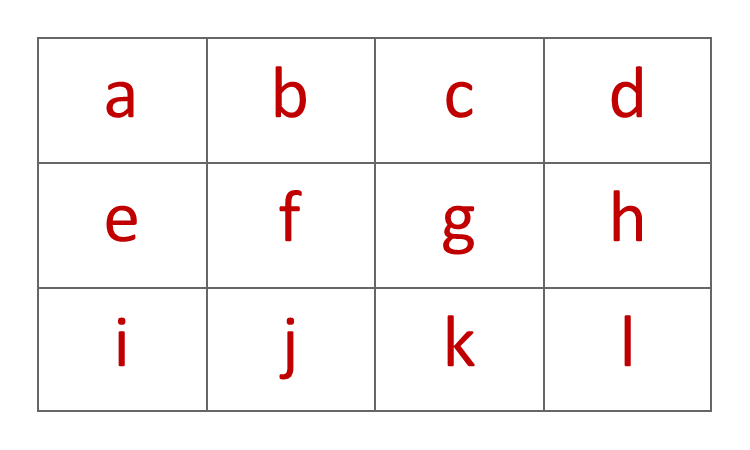
\includegraphics[scale=0.6]{../figures/2DConvExample(a)}
\caption{Input Activations}
\end{subfigure}
\begin{subfigure}{0.45\textwidth}
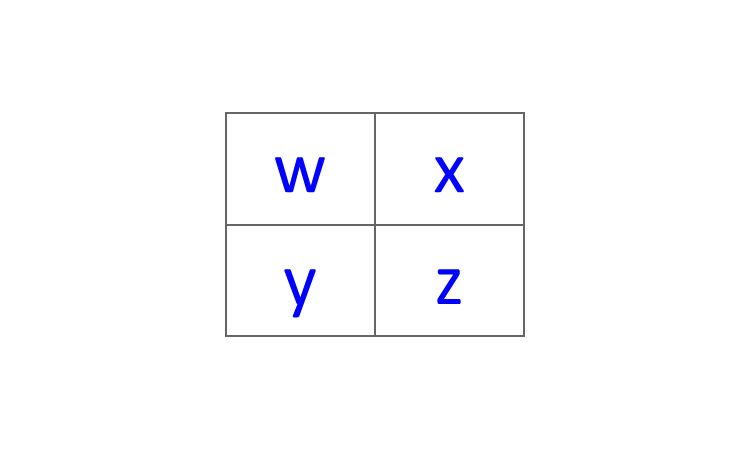
\includegraphics[scale=0.6]{../figures/2DConvExample(b)}
\caption{Convolution Filter}
\end{subfigure}
\begin{subfigure}{0.9\textwidth}
\centering
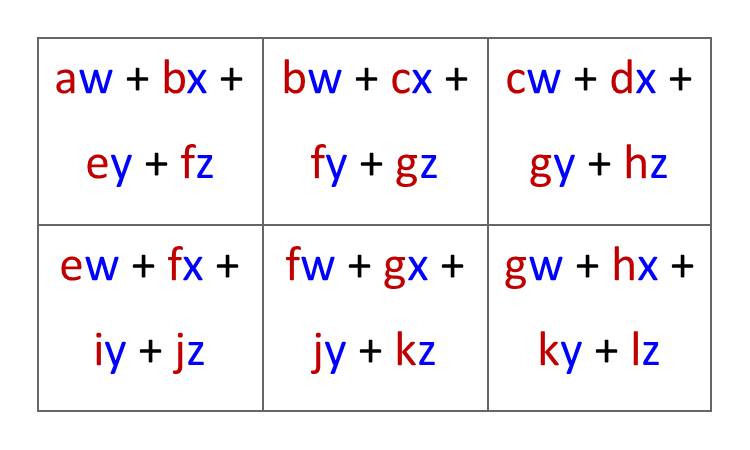
\includegraphics[scale=0.6]{../figures/2DConvExample(c)}
\caption{Convolution Result}
\end{subfigure}
\end{center}
\caption{The result of convolving an input (a) with an filter map (b) is a new set of activations (c). This Image was adapted from Goodfellow, pg. 325 \cite{Goodfellow}}
\label{fig-2DConvExample}
\end{figure}
Note that formal implementations include a bias vector and an activation function.

\paragraph*{}For 2D convolution over input $x^{(l-1)}$ with feature map $W^{(l)}_k$, producing activations $x^{(l)}$, we compute the activations $x^{(l)}_{k}$ as \cite{Goodfellow}
\begin{equation}
\label{eqn-ConvFeedForward}
x^{(l)}_k = \sigma^{(l)}\bigg[ \Big( \sum_{u=0}^{m-1} \sum_{v=0}^{n-1} x^{(l-1)}(i,j) W^{(l)}_k(i - u,j - v) \Big) + b^{(l)}_k \bigg]
\end{equation}
\textcolor{red}{Please check my math here!}
This operation repeats for each of the $K$ feature maps. Each maps has it's own $n \times m$ weighting matrix and appropriately shaped bias .

\paragraph*{}The convolution layers allows for several advantages. Among these are (i) \textit{sparse-connectivity}: not every single activation (pixel) is connect to every single output pixel, so it is more computationally efficient, (ii) \textit{positional invariance}: key features can be identified regardless of where they are in the layer, and (iii.) \textit{Automatic feature detection} as the training process will update the filters to identify dominant features in the data without human instruction \cite{Geron,Goodfellow,Loy}.

% ================================

\subsubsection{2-Dimensional Maximum Pooling Layer}
\label{subsubsec-2DPool}

\paragraph*{}A Maximum Pooling layers simply returns the maximum neuron activation in a group of neurons. In the case of 2D Max Pooling, we choose a kernel size to be $m \times n$, just like in the 2D Convolution layer, and extract the maximum value in each window, and then step along accrdoing to the chosen stride size \cite{Loy,Goodfellow}.As an example, consider again figure (\ref{fig-2DConvExample}a). Using the $2 \times 2$ kernel on the $3 \times 4$ input, each box would then contain the maximum value of the input activations. We detail this in Fig. (\ref{fig-2DMaxPool}):
\begin{figure}[h]
\label{fig-2DMaxPool}
\begin{center}
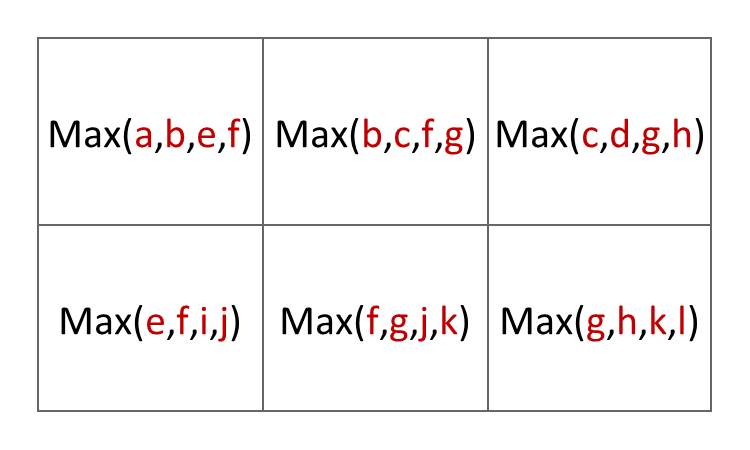
\includegraphics[scale=0.6]{../figures/2DConvExample(d)}
\end{center}
\caption{The result of 2D maximum-pooling an input array. This image was adapted from Loy, pg. 126 \cite{Loy}}
\end{figure} 

\paragraph*{}Pooling layers, such as maximum pooling, average pooling, or similar are typically placed after a layer or a set of layers of convolution. The purpose of this arrangement is to reduce the number of weights, thereby dropping the complexity of the model and ensuring only features with large activation values are preserved \cite{Geron,Loy,Goodfellow}.

% ================================

\subsubsection{1-Dimensional Flattening Layer}
\label{subsubsec-1DFlatten}

\paragraph*{}A flattening layer is used to compress an array with two or more dimensions down into a single dimension. For a flattening layer $l$, multidimensional activations in layer $l-1$ are rearranged down into a single dimensional array. Note that this is not like projecting the data into a lower dimension, but rather is simple the reorganization of values into an array of a single axis. We can use function notation to express this as:
\begin{equation}
\label{eqn-FlattenFunction}
f^{(l)} : x^{(l-1)} \in \mathbb{R}^{(M \times N \times ....)} \rightarrow
x^{(l)} \in \mathbb{R}^{(MN...\times 1)}
\end{equation}
The numerical value of each activation is left unchanged. For a layer with activation shape$N \times M$, the resulting activations are reshaped into $NM \times 1$ as shown in Eq.(\ref{eqn-FlattenFunction}).

\paragraph*{}Flattening Layer are most commonly used to prepare activations for entry into dense layer or series of dense layers. For example, 2D or 3D images are typically processed with 2D convolution, which may output a 2D or 3D array of activations. Those values are then flattened to 1 dimensions, which can then be passed into dense layers for further processing.

% ================================

\subsubsection{1-Dimensional Concatenation Layer}
\label{subsubsec-1DConcat}

\paragraph*{}The 1-Dimensional Concatenation Layer, also called 1D-Concat layer takes separate vectors of activations and combines them into a single 1D vector. Consider the layer activations $\vec{a}^{(l-1)}$ and $\vec{b}^{(l-1)}$ with shapes  $1 \times \alpha$ and $1 \times \beta$ respectively. They are the outputs of two different layers:
\begin{equation}
\vec{a}^{(l-1)} = \big[ a_{0},  a_{1}, ... ,  a_{\alpha-1} \big]
\text{\hspace{1cm} and \hspace{1cm}}
\vec{b}^{(l-1)} = \big[ b_{0},  b_{1}, ... ,  b_{\beta-1} \big]
\end{equation}
The result of the concatenation is a new 1D-array, $\vec{c}^{(l)}$ with size $1 \times \alpha + \beta$:
\begin{equation}
\vec{c}^{(l)} = \big[ a_{0},  a_{1}, ... ,  a_{\alpha-1}, b_{0},  b_{1}, ... ,  b_{\beta-1} \big]
\end{equation}

\paragraph*{}We can denote this for $n$ arrays with function notation:
\begin{equation}
\label{eqn-ConcatenationFunction}
f^{(l)} : x^{(l-1)}_{a} \in \mathbb{R}^{(1 \times \alpha)} , x^{(l-1)}_{b} \in \mathbb{R}^{(1 \times \beta)} , ....  \rightarrow
x^{(l)}_{z} \in \mathbb{R}^{(1 \times \alpha + \beta + ...)}
\end{equation}
The concatenation layer is used to combine activation non-adjacent, or non-related layers into a single new layer. In this case of the model used in the project, we use it to combine the activations that result from two distinct models into a single layer that is then transformed into a final output. This process is detailed further in sec. (\ref{sec-Architecture}).

% ================================================================

\subsection{Activation Functions Used in Network Layers}
\label{sec-ActivationFunctions}

\paragraph*{}Activation functions are a key parameter in the behavior of neural networks. As discussed in sec. (\ref{sec-Training}) a layer function, $f^{(l)}$ is generally composed of a linear transformation, as in Eq. (\ref{eqn-LinearTransform}), and then an element-wise activation function as in Eq. (\ref{eqn-elementActivation}). It is this second step that allows for neural networks to model the incredibly complex decision boundaries that are found in real-world problems \cite{Geron,Loy}. In this section, we detail the activation functions used in out classification neural network. 

\subsubsection{Rectified Linear Unit}

\paragraph*{}The Rectified Linear Unit (ReLU) activation function acts element-wise on the activations in a given layer. If the activation of a neurons is non-zero or non-negative, the value is untouched, otherwise a $0$ is returned. For an input activation $x$, ReLU is defined by:
\begin{equation}
\label{eqn-ReLU}
\text{ReLU}\big[x\big] = \max\big(0,x\big) = \left\{
\begin{array}{ll}
    x & \text{if\hspace{0.5cm}} x > 0 \\
    0 & \text{otherwise}
\end{array} 
\right.
\end{equation}
ReLU is only defined on a real domain. We provide a visualization of the function in Fig. (\ref{fig-ReLU}).
\begin{figure}[H]
\begin{center}
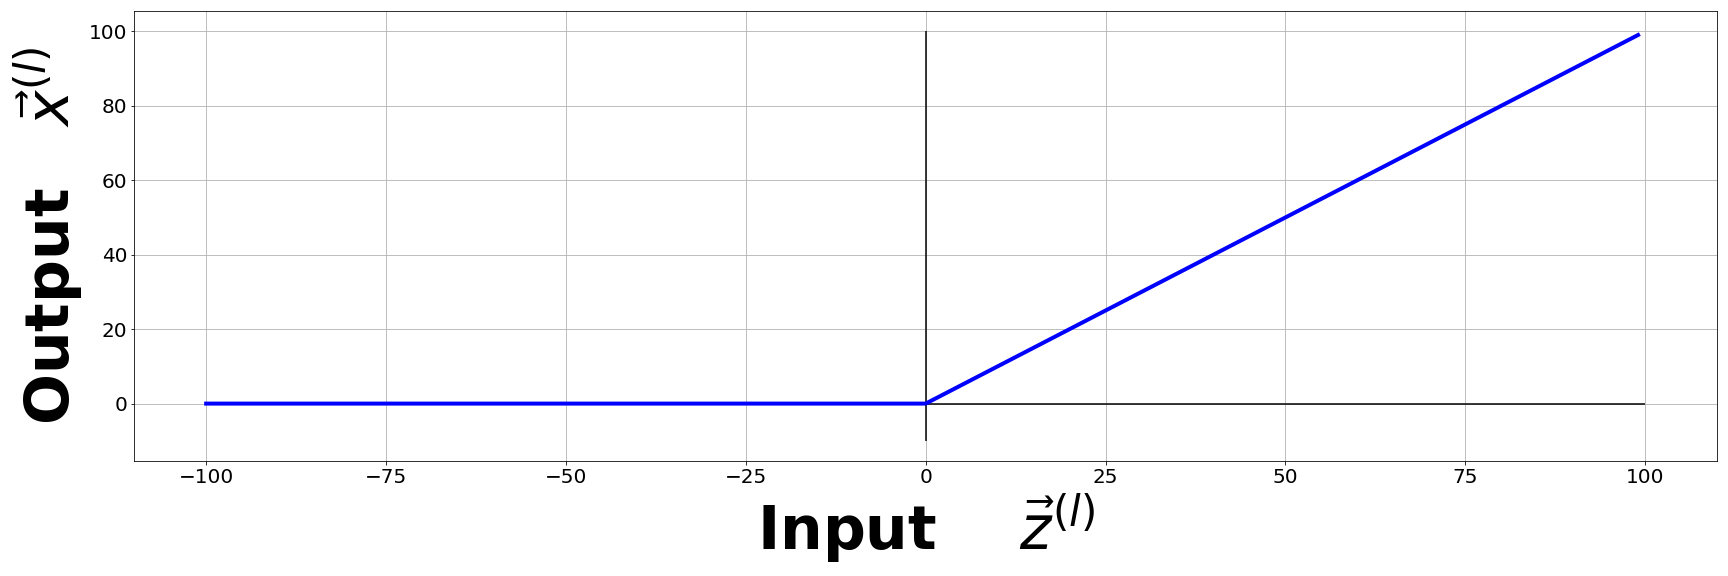
\includegraphics[scale=0.2]{../Figures/RectifiedLinearUnit}
\end{center}
\caption{Rectifed Linear Unit (ReLU) activation function}
\label{fig-ReLU}
\end{figure}
For our chosen architecture, ReLU is applied to the activations in every single Convolution layer and Dense Layer, with the exception of the output dense layer.

% ================================

\subsubsection{Softmax}
\label{subsubsec-Softmax}

\paragraph*{}The softmax activation function is commonly used in the output layer of a multi-class classification network, such as the one we implement. When softmax acts on a vector or activation, the result a non-negative output vector. with an $L_1$ norm of $1$ \cite{Geron,Goodfellow,Virtanen}. The $i$-th element in a softmax activation function is given by:
\begin{equation}
\label{eqn-Softmax}
\text{Softmax}\big[ x \big]_{i} = \frac{e^{x_i}}{\sum_{j}e^{x_j}}
\end{equation}

\paragraph*{}This function is almost only used in the output layer of a neural network, and encodes a discrete categorical probability. For example, if Eq.(\ref{eqn-Softmax}) returns a vector of the form: $[ 0.75 , 0.25]$, we interpret this as a sample having a $75\%$ chance of beloinging to class $0$ and a $25\%$ change of belonging to class $1$.


% ================================================================

\subsection{Training a Neural Network}
\label{subsec-Training}

\paragraph*{}A neural network's purpose is to produce a function $F^*$ that approximates an unknown function $F$, using a set of parameters, $\Theta$. The model must have a procedure for updating the parameters in $\Theta$ to allow for a reasonably close approximation of $F$. To better understand this, we turn to Tom Mitchell's explanation of a learning algorithm \cite{Goodfellow,Mitchell}:
\begin{quote}
A computer program is said to learn from experience $E$ with respect to some class of tasks $T$ and performance measure $P$, if it's performance at tasks in $T$, as measured by $P$, improves with experience $E$.
\end{quote}
Without any direct human intervention, a model must update itself to improve it's performance at a give task a new information is presented to it. To do this, the model must be constructed with a training procedure in mind. 

\paragraph*{}We consider the set of parameters $\Theta$ as a concatenation of each applicable layer's weighting matrix and bias vector such that:
\begin{equation}
\label{eqn-Theta}
\Theta = \big\{
W^{(0)}, b^{(0)}, W^{(1)}, b^{(1)}, W^{(2)}, b^{(2)}, ... ,W^{(L-2)}, b^{(L-2)}, W^{(L)}, b^{(L-1)},
\big\}
\end{equation}
Each parameter is floating-point number, which is stored in a weight matrix $W^{(l)}$ or bias vector $b^{(l)}$. Each value for each parameter contributes to the output of the function, thus indirectly influences the final layer activations. Note that $W^{(l)}$ or $b^{(l)}$, themselves are not parameters, but arrays of parameters to be trained. Certain layers, such as pooling layers (\ref{subsubsec-2DPooling}), concatenation layers (\ref{subsubsec-1DConcat}), or flattening layers (\ref{subsubsec-1DFlatten}) do not contain any trainable parameters. Similarly, activation functions themselves are static and are not included in the list of parameters.

\paragraph*{}In increasingly complicated neural networks, there can be upwards of hundreds of thousands,or even millions of elements in $\Theta$ making a neural network a functions that exist is a very high dimensional parameter-space \cite{Geron,Goodfellow,Levine}. For the network that we have designed in this project, there are roughly $33,000$ parameters across $20$ layers.

\subsubsection{The Cost Function}

\paragraph*{}Suppose we pass a training sample, given by the feature-vector $x^{(0)}$, with an expected outcome given by the one-hot-encoded vector $y$, into the neural network. After the network finishes processing, it's output activations are given by the vector $x^{(L-1)}$, also noted as $y^*$. For a reasonably trained model, we expect the vector $y^*$ to be "similar" to $y$, indicating that with the provided data, the network has made a valid prediction. Conversely, for an untrained network, $y^*$ is not likely to be "similar" to $y$ at all, indicating that the network has made a poor prediction. 

\paragraph*{}To quantify the difference between the model's prediction, $y^*$ and the expected output, $y$, we introduce a \textit{cost function}, $J(y^*,y)$, to the model \cite{Goodfellow,James}. The cost function, also called a \textit{loss} or \textit{objective} function, compares the neural networks output, $y^*$ and the expected output $y$. It returns a single floating-point number which measures the \textit{poorness} of the prediction. A high cost value indicates a \textit{poor} prediction, and a low cost indicates a reasonable prediction. 

\paragraph*{}$J(y^*,y)$ can take many forms and is often dependent on particular task or data set provided \cite{James}. For this $k$-classes classification task, we choose to use the \textit{Categorical Crossentropy} (CXE) cost function. For a sample labeled by the one-hot-encoded vector $y$ and corresponding prediction vector $y^*$, the CXE cost for a single sample is given by \cite{Goodfellow,Virtanen}:
\begin{equation}
\label{eqn-CXELoss}
\text{CXE}\big[ y , y^* \big] = - \sum_{i=0}^{k-1} y_i \log_{10}(y^*_i) 
\end{equation}
Thus, the average loss over a mini-batch of $b$ samples is given:
\begin{equation}
\label{eqn-CXELossAvg}
\big\langle \text{CXE}\big[ y , y^* \big]\big\rangle = 
- \frac{1}{b}\sum_{n=0}^{b-1}\sum_{i=0}^{k-1} y_i^{(n)} \log_{10}(y^{*(n)}_i) 
\end{equation}

\paragraph*{}Suppose that a given sample belongs to class $j$ in a $k$-classes classifier. Since the label vector, $y$ is one-hot-encoded, all entries are zero except $y_{j} = 1$.
\begin{equation}
y = \big[y_0,y_1, ... , y_{j} , ..., y_{k-1} \big]^T  = 
\big[0,0, ... , 1 , ...,0 \big]^T
\end{equation}
Thus the sum in Eq. (\ref{eqn-CXELoss}) contains mostly zero terms. The only non-zero term is the produce of $y_j$ and $\log_{10}(y^*_j)$. Since the vector $y^*$ has been subject to the softmax activation function, we must have $y^*_j \in [0,1]$. This means that taking the log of this value returns a negative number. Multiplying by negative number returns a high loss when the activation of $y^*_j$ is low and a low cost when $y^*_j \approx 1$. We visualize this relationship in Fig. (\ref{fig-CXELoss}):

\begin{figure}[h]
\begin{center}
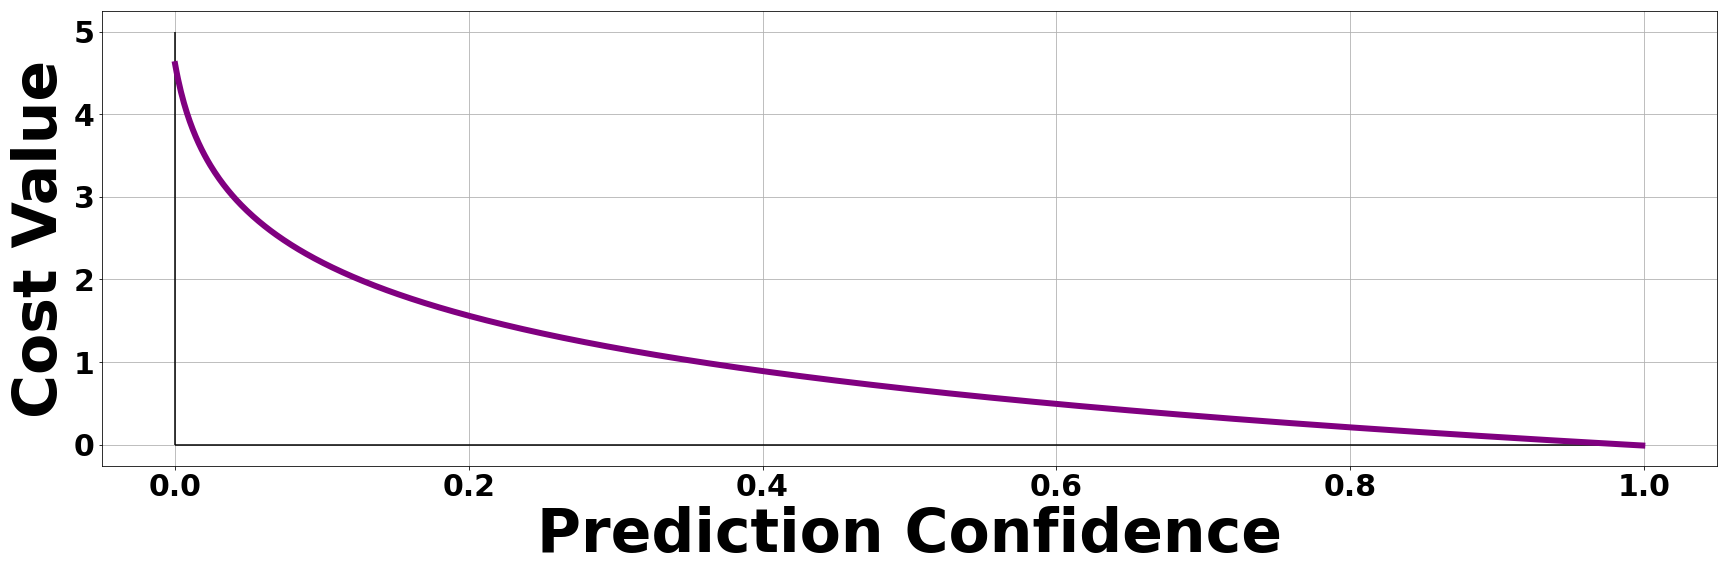
\includegraphics[scale=0.25]{../Figures/CXELoss}
\end{center}
\caption{Plot of how $y^*_{j}$ affects the output values of the CXE cost function}
\label{fig-CXELoss}
\end{figure}

\paragraph*{}By optimizing the parameters $\Theta$ in the network model, we allow for the output of a consistently low cost function to be produced across all samples in the data set.

% ================================

\subsubsection{Gradient Based Learning}

\paragraph*{}We have developed a method for quantifying the difference between a given output $y^*$ and an expected output $y$ with the inclusion of a cost function. For a trained neural network, we expect that samples consistently produce a low cost value, particularly on previous unseen inputs, which indicates that the model has appropriately \textit{generalized} \cite{James,Loy}. The process of training the model is to choose the parameters in $\Theta$ that allows for this behavior of the cost function. We then treat the training process of a neural network as a higher dimensional \textit{optimization} problem \cite{Goodfellow}.

\paragraph*{}A neural network uses \textit{indirect optimization}, which contrasts from pure optimization. Deep Learning expert Ian Goodfellow described this \cite{Goodfellow}:
\begin{quote}
In most learning scenarios, we care about some performance measure $P$,... We reduce a different cost function, $J(\theta)$ in the hope that doing so will also improve $P$.
\end{quote}
By choosing an appropriate cost function, and selecting the parameters $\Theta$ that minimize the average cost over a data set, we also assume that doing so minimizes classification error and maximizes the performance $P$.

\paragraph*{}The cost of a sample is dependent on training labels $y$ and the network output $y^*$. The output is given by the final layer activation $x^{(L-1)}$, which in turn are produced by the previous layer and so forth, as demonstrated in Eq. (\ref{eqn-altLayerFunction}), This recursive nature combined with the dimensionality of the parameter object $\Theta$ makes an analytical solution to the optimization impractical \cite{Geron,Goodfellow,James}. We instead optimize the cost function with a gradient-based method. 

\paragraph*{}We can reduce the cost given a set of parameters, $J(\Theta)$, by moving each element in $\Theta$ with small steps in the direction of the negative partial derivative of each parameter. In the case of the high-dimensional $\Theta$ object, we compute the partial derivative with respect to each weight and bias in the form of the \textit{gradient vector}. We denote the gradient of $J$ with respect to the parameters in $\Theta$ as:
\begin{equation}
\label{eqn-CostGradient}
\nabla_{\Theta}\big[ J \big] = 
\Big[ 	\frac{\partial J}{\partial W^{(0)}}, \frac{\partial J}{\partial b^{(0)}}, 
		\frac{\partial J}{\partial W^{(1)}}, \frac{\partial J}{\partial b^{(1)}}, \hdots ,
		\frac{\partial J}{\partial W^{(L-1)}}, \frac{\partial J}{\partial b^{(L-1)}} \Big]^T
\end{equation}
Where $\frac{\partial J}{\partial W^{(l)}}$ is taking the partial derivative of each element in the $W^{(l)}$ matrix, and preserves the shape.

\paragraph*{}Due to the nested composition of the network output in Eq. (\ref{eqn-FunctionChain}), and subsequently the cost itself, we must use the chain rule of calculus to work backwards through computational graph of the neural network to compute the partial derivative with respect to each parameter in $\Theta$. The process of working backwards to compute each element in the gradient vector is called \textit{back-propagation} \cite{Geron}. Below we detail an algorithm in pseudo-code to back-propagate through a fully-connected neural network, such as the multilayer perceptron outlines in sec.(\ref{sec-NetworkStructre})

\begin{algorithm}[H]
\caption{Backwards propagation system, in a standard densely connected deep neural network. Each iteration in the \textit{for-loop} computes the gradient of the cost function $J$ with respect to the weight and bias arrays. Each element in those arrays is then the discrete gradient of that parameter. A practical application of this algorithm should include batches of samples instead of a single sample}
\label{algBackProp}

\begin{algorithmic}
\REQUIRE Cost/Objective function $J$ and learning rate $\alpha$
\REQUIRE Set of weighting parameters - $W^{(i)}, i \in \{0,1,....,L-1\}$
\REQUIRE Set of bias parameters - $b^{(i)}, i \in \{0,1,....,L-1\}$
\REQUIRE Set of layer activation function - $\sigma^{(i)}, i \in \{0,1,....,L-1\}$
\REQUIRE Set of layer activation function derivatives - $\partial\sigma^{(i)}, i \in \{0,1,....,L-1\}$
\REQUIRE Set of pre-nonlinear activation - $Z^{(i)}, i \in \{0,1,....,L-1\}$
\REQUIRE Set of post-nonlinear activation - $X^{(i)}, i \in \{0,1,....,L-1\}$

Execute forward pass in algorithm (\ref{algFeedForward}) and compute the gradient of the cost with respect to the final layer activations \\
$dx \leftarrow \nabla_{(y^*)}J(y,y^*)$ \\
Initialize $\nabla J$ as output object, should have same shape as $\Theta$

\FOR {$L-1,L-2,...,2,1$}
	\item Compute gradient w.r.t pre-nonlinear activation portion of layer function
	\item $dx^{(l)} \leftarrow \nabla_{Z^{(l)}}J = dx^{(l)} \odot \partial\sigma^{(l)}[ Z^{(l)} ]$
	\item Compute gradient w.r.t weighting and bias elements
	\item $db \leftarrow \nabla_{b^{(l)}}J = dx^{(l)}$
	\item $dW \leftarrow \nabla_{W^{(l)}}J = dx^{(l)} \cdot X^{(l-1)}$

	\item Add $db$ and $dW$ steps to $\nabla J$ object
	\item $\nabla J = \nabla J .Add(dW,db)$
\ENDFOR

\item Return gradient w.r.t to each parameter in $\Theta$
\RETURN $\nabla J$

\end{algorithmic}
\end{algorithm}

\paragraph*{}After (i) computing the gradient, we can scale it by a desired learning rate, $\alpha$ and (ii) add the gradient vector element-wise to the existing elements in $\Theta$ object. By repeating steps (i) and (ii) in succession, we gradually drive the cost function to produces consistently lower and lower values across a data set \cite{Geron}. This is called \textit{gradient descent} and is the basis for many optimization algorithms. We show the general update rule on iteration $(i)$ for gradient based learning over a batch of $m$ samples in Eq. (\ref{eqn-GradientLearning}).
\begin{equation}
\label{eqn-GradientLearning}
\Theta^{(i)} = \Theta^{(i-1)} + (-\alpha)\frac{1}{m} \nabla_{\Theta} \Big[\sum_{n=1}^{m} J(y^{*(n)},y^{(n)}) \Big] \\
\end{equation}

% ================================

\subsubsection{The Optimizer}

\paragraph*{}An optimizer is the algorithm or procedure that is used by a machine learning model to achieve the lowest possible value of the cost function over a data set \cite{Geron}. Some models such as minimizing a \textit{mean-squared error} for linear regression model can be solve analytically, while high dimensional neural networks
Standard gradient-based learning, as given by the parameter update rule in Eq. (\ref{eqn-GradientLearning}) is cumbersome and often prone errors such as vanishing or exploding gradients. \cite{Geron,Goodfellow,Loy}. To combat this, model must often implement an algorithm that is more stable, and aggressive in it's ability to

\paragraph*{}For this project, we employ an \textit{Adaptive-Moments} optimization algorithm, also called \textit{ADAM} for short. It is a powerful optimizer with uses adaptive learning rate and momentum parameter. ADAM tracks an exponentially decaying average of past gradients, as well as exponentially decaying average of past squared gradients \cite{Geron}. This produces a far more aggressive optimizer at a higher computational cost.

\paragraph*{}This means that as the cost function iterates through each step, the effect will tend to "snowball". If the previous step was found to reduce the cost function by a large or small amount, the step size for the previous step will update accordingly. 
Note that a superscript $(i)$ or $(i-1)$ gives an iteration index, while the superscript $i$ means to raise a value to the power of $i$. For a given step $(i)$, The ADAM update is given:
\begin{equation}
\label{eqn-ADAMupdate}
\begin{split}
s^{(i)} &= \rho_1 s^{(i-1)} + (1 - \rho_1) \frac{1}{m} \nabla_{\Theta} \Big[\sum_{n=1}^{m} J(y^{*(n)},y^{(n)}) \Big]  \\
r^{(i)} &= \rho_2 r^{(i-1)} + (1 - \rho_2) \frac{1}{m} \nabla_{\Theta} \Big[\sum_{n=1}^{m} J(y^{*(n)},y^{(n)}) \Big] \odot
							\frac{1}{m} \nabla_{\Theta} \Big[\sum_{n=1}^{m} J(y^{*(n)},y^{(n)}) \Big]  \\
s'^{(i)} &= \frac{s^{(i)}}{1-\rho_1^i} \\
r'^{(i)} &= \frac{r^{(i)}}{1-\rho_2^i} \\
\Theta^{(i)} &= \Theta^{(i-1)} + (-\alpha)\frac{s'^{(i)}}{\sqrt{r'^{(i)}}+\delta} \\
\end{split}
\end{equation}

\paragraph*{}ADAM has experimentally shown to be a very powerful and robust optimizer useful for a wide range of tasks. Because of the two decay constants $\rho_1$ and $\rho_2$, we an compound and accumulate the values of past gradients to continue to push the cost to lower and lower values, even if the magnitude of the gradient becomes very small \cite{Geron}. 

\begin{algorithm}[H]
\caption{Adaptive-Moments (ADAM) optimizer for a neural network}
\label{algAdaGrad}

\begin{algorithmic}
\REQUIRE Step size $\alpha$
\REQUIRE Small constant $\delta$ for numerical stabilization, usually about $10^{-7}$.
\REQUIRE constants $\rho_1$, $\rho_2$ used got exponential decay rates, usually $0.9$ and $0.999$ respectively.
\REQUIRE Subroutine/function to compute gradient of cost function.
\REQUIRE Mini-batch size, $m$
\REQUIRE Stopping criterion $S$

Initialize moment variables and iteration counter $s = 0$, $r = 0$, $i = 0$ \\

\WHILE {Stopping Criterion $S$ is \FALSE}
	\item Extract a mini-batch of $m$ samples from larger data set $X$. $[x^{(0)},x^{(1)},...,x^{(m-1)}]$ and corresponding target values 
	$[y^{(0)},y^{(1)},...,y^{(m-1)}]$.
	\item Compute numerical gradient estimate of each sample in batch. This can be done with standard back-propagation in algorithm (\ref{algBackProp}) and 			 	normalize by batch size $m$:
	\item $\nabla J \leftarrow \frac{1}{m} \nabla_{\Theta} \Big[\sum_{n=1}^{m} J(y^{*(n)},y^{(n)}) \Big]$
	
	\item Compute first bias moment: $s \leftarrow \rho_1 s + (1 - \rho_1) \nabla J$
	\item Compute second bias moment: $r \leftarrow \rho_2 s + (1 - \rho_2) \nabla J \odot \nabla J$
	\item First bias correction: $s' \leftarrow \frac{s}{1 - \rho_1^i}$
	\item Second bias correction: $r' \leftarrow \frac{r}{1 - \rho_2^i}$
	
	\item Compute And Apply update:	$\Delta \Theta = (-\alpha) \frac{s'}{\sqrt{r'} + \delta}$
	\item $\Theta = \Theta + \Delta \Theta$	
	\item Update Iteration number: $i \leftarrow i + 1$
\ENDWHILE

\end{algorithmic}
\end{algorithm}


% ================================================================

\subsection{Chosen Model Architecture}
\label{sec-Architecture}

\paragraph*{}The success of a neural network algorithm is enormously dependent of the strength of the chosen features, as well as a complementary architecture, rather than the quantity of available data \cite{Geron,Kahn,Liu}. We have derived an appropriate set of inputs arrays, explore in sec. (\ref{sec-Features}) and constructed a neural network architecture to coincide with these features. From each sample, we produce two input arrays, one being a matrix and the other being a column-vector, and present those to a  \textit{multimodal neural network} \cite{Virtanen}. This type of hybrid network accepts one array at each of two input layers, passes them through a series of non-overlapping layers, and combines separate neural networks into a single model to produce a one prediction resulting from both inputs \textcolor{blue}{citation for multimodal networks}.

\paragraph*{}The full classification neural network used for this project consists of two distinct entry points. Rather than presenting the network with one set of input data, $X$, we present the network with two different arrays, $X_1$ and $X_2$. Both arrays are a product of the same audio file sound wave, and thus share a common training label, $y$. Each of the two entry layers leads to it's own branch and the given information is process roughly in parallel. Once a certain number of layer functions have been applied, each arm of the neural network is left with a single dense layer of activations. These two activation vectors are concatenated into a single new dense layer, and then passed through one final layer to generate the model's final output. A visual representation of this architecture can be found in Fig. (\ref{fig-NetworkArchitecture}).

\begin{figure}[H]
\label{fig-NetworkArchitecture}
\begin{center}
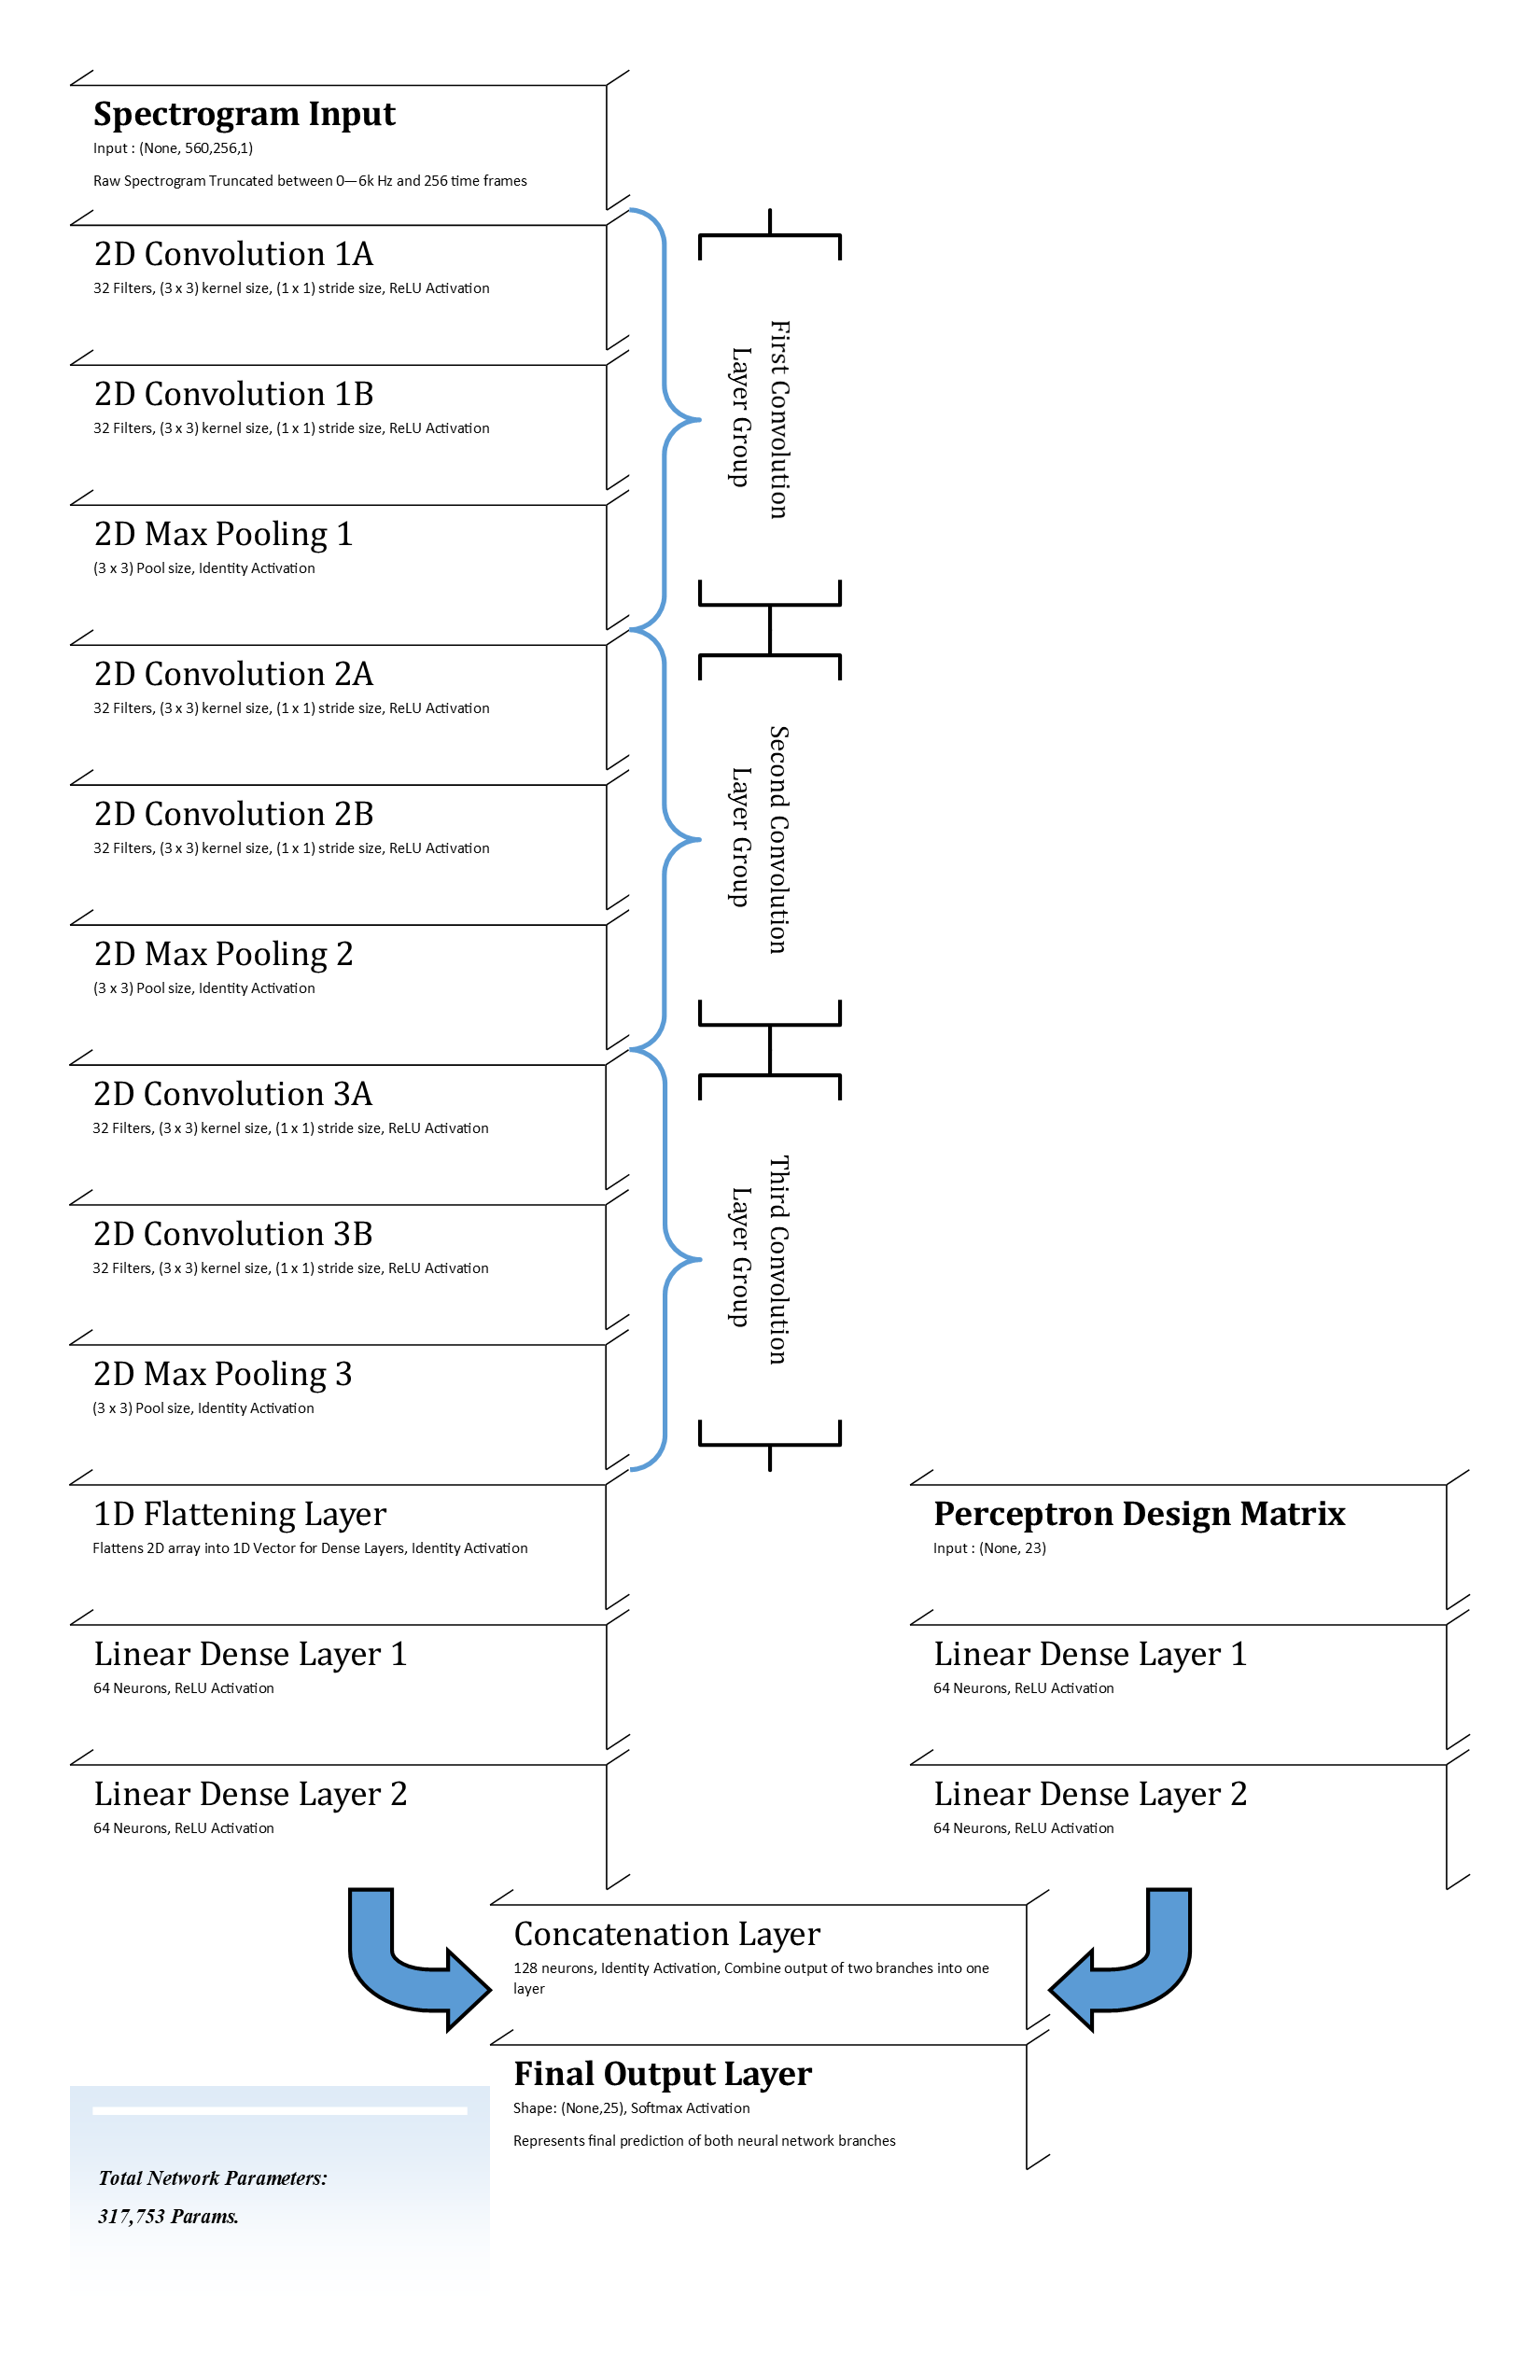
\includegraphics[scale=0.45]{../Figures/NeuralNetworkArchitecture}
\end{center}
\caption{The developed architecture of the audio file classification neural network. The Left branch process an image-like input, the right branch processes a vector-like input. The activations are then merged, and then a single output is produced}
\end{figure}

% ================================

\subsubsection{The Spectrogram Branch}

\paragraph*{}The spectrogram branch is pictured on the left side of Fig. (\ref{fig-NetworkArchitecture}). A spectrogram is a representation of a sound wave, or signal by representing energy distributions as a function of \textit{time} and \textit{frequency} \cite{White,Olsen,Kahn}. \textcolor{blue}{Details on the creating of the spectrogram can be found in the \textit{features} section of this document.}

\paragraph*{}The input layer of the spectrogram accepts a 4-Dimensional array. The axes, in order of indexing, represents (i) the size of the \textit{mini-batch} of samples, (ii) the pixel width of each sample, (iii) the pixel height of each sample, and (iv) the number of channels in each sample. As a model hyper-parameter, we have chosen each batch to contain $64$ samples. We have also chosen to truncate time and frequency axes (ii \& iii) to contain $560$ frequency bins, and $256$ time-frames. Each image also contains a single channel, which make it gray-scale when visualized. We can denote the 4D shape of the input object into this branch as:
\begin{equation}
\label{eqn-shapeX1}
X_1 \in \mathbb{R}^{(64 \times 560 \times 256 \times 1)}
\end{equation}
Any other shape will be rejected by the model, and an error is raised.

\paragraph*{}After the input layer assert the appropriate shape, the array $X_1$, which is a collection of $64$ spectrograms, is passed into the first of three \textit{Convolution Layer Groups}. These layer groups are inspired from the \textit{VGG-16 Neural Network} architecture \textcolor{red}{[citation needed]}. Each convolution layer group in composed of three individual layers: 
\begin{enumerate}
\item A 2-Dimensional Convolution layer, using $32$ filters, a $3 \times 3$ kernel, a $1 \times 1$ step size, and a ReLU activation function,
\item A 2-Dimensional Convolution layer, using $32$ filters, a $3 \times 3$ kernel, a $1 \times 1$ step size, and a ReLU activation function,
\item A 2-Dimensional Maximum Pooling layer using a $3 \times 3$ pooling size, and an Identity activation function
\end{enumerate}  
The Convolution layers convoluted over the middle two axes of the data (over space and time in the spectrogram). 

\paragraph*{}By grouping layers in this structure, we use the convolution  layers to reduce the number of features, and then the pooling layer to extract only the largest activations of the remianing features. This ensures that in the full spectrogram image, only the dominant features and feature shapes are preserved and passed into the next layer set for processing.

% ================

\subsubsection{The Perceptron Branch}

\paragraph*{} The Perceptron branch is picture on the right side of Fig. (\ref{fig-NetworkArchitecture}), notice that it is considerably smaller in side and complexity than it's neighbor. Rather than accept an image-like input, the perception simply takes a vector-like input of properties that are derived from the audio file. We call these properties \textit{features} \cite{Geron,Kahn,Serizel}. \textcolor{blue}{Details on the creating of these features can be found in the \textit{features} section of this document.}

\paragraph*{}The input layer of the perceptron accepts a 2-Dimensional array. The axes, in order of indexing, represent (i) the size of the \textit{mini-batch} of samples, (ii) the number of features for each sample. We use the same model hyper-parameter of $64$ samples per batch, and have developed $20$ unique classification features that have been derived from time-space and frequency-space representations of the audio file data. We can denote the 2D shape if the input object into this branch as:
\begin{equation}
\label{eqn-shapeX2}
X_2 \in \mathbb{R}^{(64 \times 20)}
\end{equation}
This 2D is referred to as a \textit{design matrix} \cite{James,Loy}. Any other shape will be rejected by the model, and an error is raised.

\paragraph*{}In perceptron models, scaling the design matrix appropriately drastically improves the classification performance. A design matrix is scaled by taking all samples in a column (a particular feature from each class), subtracting the average, and then scaling it such that it has unit variance \cite{Geron,James}. This ensures that no one feature dominates the performance of the model and that layer activations to not get saturated as data progresses through the network.

% ================

\subsubsection{The Final Output Branch}

\paragraph*{}The last layer in each of the two branches is a ReLU-activated Dense layer containing 64 neurons, represented by a $64 \times 1$ column vectors. We combine these model layers by using a \textit{concatenation layer} to fuse the two column vectors together, "vertically", such that the result is a $128 \times 1$ column vector. This vector is then passed into the final dense layer, which used the softmax activation, and encodes the joint predictions based on both model branches. 

% ================================================================
% ================================================================

\newpage
\section{Properties of Musical Instruments}
\label{sec-Instruments}

\paragraph*{}As discussed in Sec. (\ref{sec-TheNeuralNetwork}), performance quality of a neural network is greatly dependent on the properties of the chosen features \cite{Virtanen,Liu}. To ensure that a the classifier model performs adequately and consistently, we must choose these features to have high variance between classes, and low variance within each class. This enables a neural network to development clear decision boundaries between each unique class \cite{James,Serizel}. To develop this set of features, we explore the physical and mechanical properties of musical instruments and the sounds that they create.

\paragraph*{}We have assembled training data samples than can be grouping in 38 classes of unique sources listed below:
\begin{multicols}{2}
\begin{enumerate}
	\item Alto Flute
	\item Alto Saxophone
	\item Banjo
	\item Bass
	\item Bass Clairnet
	\item Bass Flute
	\item Bassoon
	\item Bass Tromobe
	\item B$\flat$ Clarinet
	\item Bells
		
	\item Cello
	\item Clarinet \textcolor{blue}{Check this!}
	\item Contrabassoon
	\item Crotale
	\item E$\flat$ Clarinet
	\item English Horn
	\item Flute
	\item Guitar
	\item Hi-Hat
	\item Horn
		\columnbreak
	\item Mandolin
	\item Marimba
	\item Oboe
	\item Sawtooth Wave
	\item Saxophone (Tenor)
	\item Sine Wave
	\item Soprano Saxophone
	\item Square Wave
	\item Tenor Trombone
	\item Triangle Wave
		
	\item Trombone
	\item Trumpet (B$\flat$)
	\item Tuba
	\item Vibraphone
	\item Violin
	\item Viola
	\item White Noise
	\item Xylophone
	\item
	\item
\end{enumerate}
\end{multicols}

\paragraph*{}Rather than explore each class individually, we can examine the properties of groupings of musical instrumentsby using the \textit{Hornbostel-Sachs} system \textit{red}{Citation needed!}. In this syetem, musical instruments or sound sources can be divided up into four broad categories based on the nature of the sound-producing material. These categories are (i) idiophones, (ii) membranophones, (iii) chordophones, and (iv) aerophones. In this section, we explore the mechanical properties of each group and show how the physics of the source instrument influences our feature choice.


% ================================================================

\subsection{Idiophones}
\label{subsec-Idiophone}

\paragraph*{}An idiophone is an instrument that produces sound through the vibration of the full body of the object. This generally includes most percussive instruments excluding drums \textcolor{red}{citation needed}. From the set of classes that we use, bells, crotales, Hi-hats, vibraphones, and xylophones are all examples of idiophones. 

% ================================================================

\subsection{Membranophones}
\label{subsec-membranophones}

% ================================================================

\subsection{Chordophones}
\label{subsec-chordophones}

\paragraph*{}A chordophone is a musical instrument that produces sound through the vibration of strings that are stretched between two fixed points \textcolor{red}{citation needed}. From our data set, banjos, basses, cellos, guitars, mandolins, violins, and violas are all examples of chordophones.

\subsubsection{The 1-Dimension Vibrating String}

\paragraph*{}We can model a chordophone as having a string of length $L$, with a constant linear mass density, $\mu$, subject to a tension force $F_T$. The string is flexible, and free to vibrate in a single dimension. We describe the state of string over space and time with a function $U(x,t)$. The behavior of the string can be  modeled by D'Alembert's 1-dimensional wave equation \cite{Haberman,Taylor}:
\begin{equation}
\label{eqn-1DWaveEqn}
\frac{\partial^2 U}{\partial t^2} = v^2 \frac{\partial^2 U}{\partial x^2}
\end{equation}
Where $v$ is the wave propagation velocity, given by $\sqrt{\frac{F_T}{\mu}}$. Additionally, the string is fixed in place at both ends, which can be modeled by the boundary conditions:
\begin{equation}
U(0,t) = 0 
	\text{\hspace*{2cm} and \hspace*{2cm}}
U(L,t) = 0 
\end{equation}

\paragraph*{}In order to specify a solution, we must also specificy two intitial conditions. We described the initial state of the string at time $t = 0$  by the two conditions:
\begin{equation}
U(x,0) = f(x) 
	\text{\hspace*{2cm} and \hspace*{2cm}}
\frac{\partial U}{\partial t}(x,0) = g(x)
\end{equation}
Depending on the exact nature of the source instrument, $f(x)$ and $g(x)$ can take on different forms. For example, for plucked stringed instruments, $f(x)$ may appear to be as triangle-like function, with a peak at some position $0 < x_0 < L$ where then string was struck. $g(x)$

\paragraph*{}We explore solutions that take the form \cite{Haberman}:
\begin{equation}
U(x,t) = \psi(x)h(t)
\end{equation}
From this separation, we find that $\psi(x)$ and $h(t)$ each are composed of a linear combination of orthogonal trigonometric functions. Applying the boundary and initial conditions to the system allows for a linear combination of solutions \cite{Haberman}:
\begin{equation}
U(x,t) = 
\sum_{n=1}^{\infty} \bigg( A_n \sin\big(\frac{n\pi x}{L}\big)\cos\big(\frac{n\pi vt}{L}\big)
+ B_n \sin\big(\frac{n\pi x}{L}\big)\sin\big(\frac{n\pi vt}{L}\big) \bigg)
\end{equation}
The initial conditions are satisfied if:
\begin{equation}
\begin{array}{ll}
    f(x) = \sum_{n=1}^{\infty} A_n \sin\big(\frac{n\pi x}{L}\big) \\
    g(x) = \sum_{n=1}^{\infty} B_n\big(\frac{n\pi v}{L}\big)
    			\sin\big(\frac{n\pi x}{L}\big)
\end{array} 
\end{equation}
Where $A_n$ and $B_n$ are given by:
\begin{equation}
\begin{array}{ll}
    A_n = \frac{2}{L} \int_{0}^{L} f(x) \sin\big(\frac{n\pi x}{L}\big) dx \\
    B_n = \frac{2}{n\pi v} \int_{0}^{L} g(x) \sin\big(\frac{n\pi x}{L}\big) dx \\
\end{array} 
\end{equation} 

\subsubsection{Consequences of the Wave Equation}

\paragraph*{}The solution that we have derived from the wave equation shows that the behavior of $U(x,t)$ is greatly dependent on the nature of the string's initial shape, $f(x)$, when struck. In the case of picked or plucked instruments, the initial shape of $f(x)$ would be something like a "ramp function":
\begin{equation}
\label{eqn-RampFunc}
f(x) = 
\end{equation}

% ================================================================

\subsection{Aerophones}
\label{subsec-Aerophones}

% ================================================================

\subsection{Other Generated Sounds}
\label{subsec-Generated}

\paragraph*{}We group sounds produced from non-physical musical instruments in this final category. Form our data set, this category includes the four simplest waveforms, (i) sine waves, (ii) sawtooth waves, (iii) square waves, and (iv) triangle waves, as well as any color noises \cite{White}. Since these sounds are only produced synthetically through a MATLAB program, we choose not to include them in the Hornbostel-Sachs grouping above. We explore the properties of each of these generated sounds.

% ================

\subsubsection{Sine Wave}

\paragraph*{}A sine wave is the simplest of sound waves, and makes up the foundation for all periodic wave forms \cite{White,Virtanen}. It consists of a single oscillatory term with a fixed fundamental frequency $f_0$. A sine wave's amplitude as a function of time is given by 
\begin{equation}
\label{eqn-SineWave}
x(t) = A_0 \sin(2\pi f_0 t + \phi)
\end{equation}
Where $A_0$ gives an amplitude, $f_0$ is the fundamental frequency, and $\phi$ is a phase shift. We show a simple sine wave in the time and frequency domain in Fig. (\ref{fig-SineWave}).

\begin{figure}[h]
\begin{center}
	\textit{[Image of Sine Wave Waveform]}
	\textit{[Image of Sine Wave Freq. Spect]}
\end{center}
\caption{A sine wave in the (a) time-domian and (b) frequency domain}
\label{fig-SineWave}
\end{figure} 

\paragraph*{}A pure sine wave contains no overtones, only a time-independent fundamental frequency, which can take on any value due to synthetic generation.

% ================

\subsubsection{Sawtooth Wave}

\paragraph*{}

% ================

\subsubsection{Square Wave}

\paragraph*{}A square wave is a piece-wise defined waveform whose value alternatively alternates between $+1$ and $-1$ \cite{White,Olsen}. A square wave with period $f_0$ has a waveform defined over a single period as:
\begin{equation}
\label{eqn-SquareWave}
x(t) =  \left\{
\begin{array}{ll}
    +1 & \text{\hspace{0.5cm}} 0 < x \leq T_0 / 2 \\
    -1 & \text{\hspace{0.5cm}} T_0/2 < x < T_0
\end{array} 
\right.
\end{equation}
where $T_0 \equiv 1/f_0$.

\paragraph*{}We can use Fourier decomposition to examine the constituent sinusoidal wave that make up a square wave. The frequency space representation of a square wave indicates that is can be approximated as a sum of higher odd-numbered harmonics, with the amplitude of each decreasing by the reciprocal of the harmonic number \cite{White}. Thus a square wave in the time domain can be approximated as:
\begin{equation}
x(t) \approx \sum_{n = 1}^{\infty} \frac{1}{2n-1} \sin \bigg( 2 \pi (2n - 1)f_0 t \bigg)
\end{equation} 

\begin{figure}[h]
\begin{center}
	\textit{[Image of Square Wave Waveform]}
	\textit{[Image of Sqaure Wave Freq. Spect]}
\end{center}
\caption{A square wave in the (a) time-domain and (b) frequency domain}
\label{fig-SquareWave}
\end{figure}

% ================

\subsubsection{Triangle Wave}

% ================

\subsubsection{White Noise}


% ================================================================
% ================================================================

\newpage
\section{Feature Selections}
\label{sec-Features}

\paragraph*{}Classification tasks require a set of inputs that are used to make the decision as to which class the sample belongs to. These inputs are called \textit{predictors} or \textit{features} \cite{James,Loy,Serizel}. Features are quantitative, low-dimensional representations of each sample that convey key characteristics of the sample. 
Audio machine learning researchers M. Kashif Saeed Khan and Wasfi G. Al-Khatib discusses the vitality of feature selection \cite{Khan}:
\begin{quote}
The data reduction stage which is also called feature extraction, consists of discovering a few important facts about each class. The choice of features is critical as it greatly affects the accuracy of audio classification. 
\end{quote}
In the case of the biological process, the features of the audio is simply the raw time series waveform as processed by the brain. This information is then used into categorize the source. In the case of the neural network model, the time series waveform alone has shown to be unreliable in classification tasks \cite{Serizel}. We must then develop a set of features or predictors that can describe important properties of the waveform in a far more efficient manner \cite{Goodfellow,James}.

\paragraph*{}It becomes quickly apparent that the choice of features is extraordinarily important to the process of training and evaluation of the classifier model. Consider the task of identifying cats and dogs from images, given only images consisting of the top-most row of pixels. The inappropriate choice features does not reflect the significant characteristics of the data.

\paragraph*{}Tuomas Virtanen, machine learning and audio engineer writes in his book, "Computational Analysis of Sound Scene and Events" about specifically how features must be chosen \cite{Virtanen}:
\begin{quote}
For recognition algorithms, the necessary property of the acoustic features is low variability among features extracted from examples assigned to the same class, and at the same time high variability allowing distinction between features extracted from examples assigned to different classes.
\end{quote}
To ensure the construction of a suitable model, we derive features based from three representations of the audio file: (i) a spectrogram matrix of the waveform, (ii) the time-space representation of the waveform, and (iii) the frequency-space representation of the waveform. It is important to note that although this algorithm will classify sound data to instruments, the model will never actually be presented with a waveform directly, instead it will rely solely on the features.

\paragraph*{}To ensure suitable performance of this sound wave classification neural network, a great deal of time has been devoted to the construction of the elements of the feature vector. These features are derived are principles of music, digital signal processing, previous work, and underlying physics that governs the behavior of instruments. In the following sections, we outline the set of $21$ features used in the classification process. For each feature, we visualize the distribution in across each class in the form as box-plots. Each feature has been normalize to have a zero mean, and unit-variance acorss all classes. 

\newpage

% ================================

\subsubsection{The Design Matrix}

\paragraph*{}The spectrogram and $20$ features from each sample are organized into one of two array structures, each called a \textit{design matrix}. A design matrix contains real floating-point numbers that stores the features in a convenient way for the neural network to digest. For this hybrid neural-network, we use two matrices, $X_1$ and $X_2$, each containing data from $b$ audio file samples. each has shape given by:
\begin{equation}
\label{eqn-X1Shape}
X_1 \in \mathbb{R}^{(b \times N' \times k \times 1)}
\end{equation}
\begin{equation}
\label{eqn-X2Shape}
X_2 \in \mathbb{R}^{(b \times p)}
\end{equation}
Where $N' \times k \times 1$ gives the shape of a single spectrogram matrix $S$, described in sect. (\ref{subsec-spectrogram}). Similarly, $p$ is the number of features derived from the time and frequency-representation of features outlined in sec. (\ref{subsec-time}) and sec.(\ref{subsec-frequency}).The first axis, with size $b$ indicates that there are $b$ audio samples stored in that design matrix.

% ================================

\subsubsection{Audio Preprocessing}
\label{subsubsec-Preprocessing}

\paragraph*{}Preprocessing a data set is a necessary step to execute prior to feature extraction \cite{Geron2,James}. In the case of audio files, preprocessing usually consists of ensuring that the data set contains the following:
\begin{enumerate}
\item A suitably sized number of files, of reasonable audio quality, with normalized amplitudes
\item Audio encoded in a standard, and consistent format
\item A consistent sample rate and bit depth between audio files
\item A consistent number of channels
\end{enumerate}
Note that different projects may require a different set of requirement from preprocessing \cite{Virtanen}. For this project, we have chosen to use the following parameters:
\begin{enumerate}
\item Roughly $16,000$ audio files Professionally or semi-professionally recorded in a studio. \textcolor{red}{Citation needed!}. All ampltiudes have been normalized to $\pm 1$ unit.
\item All audio has be converted into \textit{.WAV} files from other formats, such as \textit{.AIF} or \textit{.MP3} using a MATLAB program
\item All audio is sampled at $44,100$ Hz and \textcolor{blue}{Bit depth needed - 16? 24?}
\item All audio has been down-mixed into mono-channel waveforms.
\end{enumerate}

% ================================================================

\newpage

\subsection{Spectrogram Features}
\label{subsec-spectrogram}

\paragraph*{}The field of neural classification is well studied in the application of image-processing. Many large-scale, and even introductory projects find themselves under the umbrella of image classification \cite{Geron,Goodfellow,Loy,Mierswa}. As a result, model architectures for image processing related tasks are well-explored and have shown experimentally successful behavior. Following this success, it make senses to provide an image-like representation of a sound wave as a feature. We do this in the form of a spectrogram matrix.

\paragraph*{}A spectrogram is a representation of the energy distribution of a sound wave as a function of both frequency and time. In a conventional spectrogram, the passing of time is shown along the $x$-axis, and the frequency spectrum is shown on the $y$-axis. Thus each point in the 2-Dimensional space is an energy at a given time and frequency. Examples spectrograms from the wave form data set are shown in Fig. (\ref{fig-spectrograms}).

\begin{figure}[H]
\begin{center}
\label{fig-spectrograms}
\textcolor{red}{Insert spectrograms here}
\caption{Spectrogram representations of various waveforms}
\end{center}
\end{figure}

\paragraph*{}A spectrogram is produced by the method of \textit{frame-blocking}, which is very prevalent in audio signal classification \cite{Liu,Zhang}. Frame-blocking takes a raw waveform or signal, $s$ and decomposes it into a set of analysis frames, $a_i$, with each being $N$ samples in length, and has a fixed overlap with the next adjacent frame. Each of the $k$ frames then allows for a section of the signal in quazi-stationary state \cite{Kahn,Serizel}. 

\paragraph*{}For this project, we have chosen to use frames of size $N = 4096$ with a $75\%$ or $3072$ sample overlap. Since each audio file contains a different number of samples, we choose the number of frames, $k$ to be less than or equal to $256$. If $k > 256$, the waveform in truncated, if $k \leq 256$ the frames left as is. The audio has been sampled at $f_s = 44100$ samples/second, so each frame represents a slice of time that is about $0.1$ seconds long.

\paragraph*{}We concatenate each analysis frame, $a_{i}, i \in [0,k-1]$ into a single $k \times N$ matrix, called $A$. Each row is a frame, each column is an index in that frame
\begin{equation}
\label{eqn-FrameMatrix}
A = \big\{ a_{0} , a_{1} , a_{2} , ... , a_{k-1} \big\} = 
\begin{bmatrix}
a_{0}[0] & a_{0}[1] & a_{0}[2] & \hdots & a_{0}[N-1] \\
a_{1}[0] & a_{1}[1] & a_{1}[2] & \hdots & a_{1}[N-1] \\
a_{2}[0] & a_{2}[1] & a_{2}[2] & \hdots & a_{2}[N-1] \\
\vdots 		& \vdots 	  & \vdots 		& \ddots & \vdots        \\
a_{k-1}[0] & a_{k-1}[1] & a_{k-1}[2] & \hdots & a_{k-1}[N-1] \\
\end{bmatrix}
\end{equation}
We use bracket notation, $a[j]$ to indicate that each analysis frame $a_i$ is array-like. The following indexing conventions for matrix $A$ all represent the same entry:
\begin{equation}
\label{eqn-IndexingA}
A_{i,j} = A_i[j] = A[i][j] = A[i,j]
\end{equation}

\paragraph*{}After frame-blocking, we apply a \textit{windowing function} to each frame. A standard \textit{Hann Window} of $N$ samples is generated as a $1 \times N$ row-array, $H$. The $n$-th index in a Hann window with $N$ samples is defined:
\begin{equation}
\label{eqn-Hann}
H[n] = \frac{1}{2}\bigg[ 1 - \cos\Big( \frac{2\pi n}{N-1}\Big)\bigg]
\end{equation}
This window function is applied to each analysis frame by computing the element-wise product of the Hann window array, $H$ and each row of the analysis frames matrix, $A_{i,:}$. Result is an $k \times N$ array, $\widetilde{A}$:
\begin{equation}
\label{eqn-WindowMatrix}
\widetilde{A_i} = A_i \odot H
\end{equation}
The window function allows for a cleaner transform into frequency space \cite{Virtanen}. \textcolor{blue}{Expand on this. HOW? Why do we use a windowing function?}

\paragraph*{}Finally, we perform a \textit{Discrete Fourier Transform} (DFT) to bring each analysis frame from a time domain into a frequency domain \cite{Olson,Peatross}. The Discrete Fourier Transform is applied by producing an $N \times N$ \textit{transform matrix}, often noted at $\mathbb{W}$. Let $\omega^k = e^{\frac{-2\pi i}{N}k}$, then the DFT matrix for a time-space containing $N$ samples
\begin{equation}
\label{eqn-DFTMatrix}
\mathbb{W} = \frac{1}{\sqrt{N}}
\begin{bmatrix}
1 & 1 & 1 & 1 & \hdots & 1 \\
1 & \omega		& \omega^2 & \omega^3 & \hdots & \omega^{N-1} \\
1 & \omega^2	& \omega^4 & \omega^6 & \hdots & \omega^{2(N-1)} \\
1 & \omega^3	& \omega^6 & \omega^9 & \hdots & \omega^{3(N-1)} \\
\vdots & \vdots & \vdots & \vdots & \ddots & \vdots \\
1 & \omega^{N-1} & \omega^{2(N-1)} & \omega^{3(N-1)} & \hdots & \omega^{(N-1)^2}
\end{bmatrix}
\end{equation}
Each column of the matrix is a complex sinusoidal oscillating with an integer number of periods within the $N$-sample length window \cite{Short,Peatross}.The DFT is applied by a taking the matrix - product of $\mathbb{W}$ and $\widetilde{A}^T$. The transpose of $\widetilde{A}$ then makes each analysis frame into a column vector, which gives the appropriate dimension for multiplication.
\begin{equation}
\label{eqn-DFT}
\text{DFT}\big[ \widetilde{A} \big] = \mathbb{W}\widetilde{A}^T
\end{equation}

\paragraph*{}Most standard implementations of neural network models require all activations, weights, and biases to be real floating-point numbers. Since the the DFT matrix introduces complex values, we compute the square of the element-wise $L2$-norm of the resultant array.
\begin{equation}
\label{eqn-Spectrogram}
S_{i,j} = \big{\lVert} (\mathbb{W}\widetilde{A}^T)_{i,j} \big{\rVert}_{2}^{2}
\end{equation}
Where $\mathbb{W}$ is the DFT matrix from Eq. (\ref{eqn-DFTMatrix}) and $\widetilde{A}^T$ is the transpose of the analysis frames matrix from Eq. (\ref{eqn-WindowMatrix}). The matrix $S$, is the spectrogram representation of the initial waveform, and has shape $N \times k$ of real floating-point numbers. We can index matrix $S$ similarly to that of matrix $A$ in Eq. (\ref{eqn-IndexingA}):
\begin{equation}
\label{eqn-IndexingS}
S_{i,j} = S[i][j] = S[i,j]
\end{equation}

\paragraph*{}Each column of the $S$ matrix is now a single-frame that has been moved into a frequency-space representation, thus there are $k$ columns, just as there were $k$ time-series analysis frames. Given the discretized nature of digital audio, the frequency-space representation is not a continuous function, but rather a column vector, where the frequency has been assigned to one of $N$ bins, ranging from $-f_s / 2$ to $+f_s/2$. To ensure homogeneous input sizes between all samples, we zero-pad the matrix $S$ with additional columns until $k = 256$. Recall that wave forms were truncated to ensure that $k \leq 256$ analysis frames.

\paragraph*{}Standard western musical instruments seldom extend above $6$ kHz \cite{Olson,Virtanen,White}. This means that when constructing the spectrogram, we will rarely ever see energy present above this frequency at any time, and the $S$ matrix will contain mostly zero, or zero-like entries. To condense the size of the matrix, we select onlt the frequency bins that correspond to energies between $0$ Hz and $6000$ Hz. This makes the input array smaller, and eliminates redundant and non-useful information. The number rows in the $S$ matrix is reduced from $N$ down to $N'$. 

\paragraph*{}Each spectrogram is now $N' \times k \times 1$ (The last axis represents a single pixel channel, as opposed to $3$ channels for RGB inputs, etc.) and effectively encodes the energy distribution of the waveform as a function of both time and frequency. The spectrogram is the first feature used in this model. For this classifier, we have chosen $N' = 558$ and $k = 256$. For training, a batch of $b$ samples are concatenated into a single array object. For a batch of $b$ samples of $N' \times k \times 1$ spectrograms, we shape $X_1$ such that:
\begin{equation}
\label{eqn-X1 shape}
X_1 = \big\{ S^{(0)},S^{(1)},S^{(2)}, ... , S^{(b-1)} \big\} \in \mathbb{R}^{(b \times N' \times k \times 1)}
\end{equation}
Which is consistent with the shape of the $X_1$ matrix outlined in eqn(\ref{eqn-X1Shape}). This matrix is presented to the \textit{Convolution} branch of the neural network for processing.

% ================================================================

\newpage

\subsection{Time-Space Features}
\label{subsec-time}

\paragraph*{}The features described in this section are derived from time-domain representations of each audio sample.For consistency between smaples, each waveform is padded or truncated to contain exactly $M$ samples. Time space is indexed by $s[i]$ with $i \in [0,1,2,3,...,M-2,M-1]$


\paragraph*{}From time space, we use the following $7$ features:
\begin{itemize}
\item[•] Time Domain Envelope
\item[•] Zero Crossing Rate
\item[•] Temporal Center of Mass
\item[•] Auto Correlation Coefficients ($\times 4$)
\end{itemize}

% ================================

\subsubsection{Time Domain Envelope}

\paragraph*{}The time domain envelope (TDE) is a method of determining which parts of the sound wave contains most of the energy of the signal Often, we compute the RMS-Energy of each frame - a larger energy of the frame, the larger the average amplitude of the waveform in that frame. For frames with smaller amplitude, it is likely that the signal has either not begun, or is decaying. 

\paragraph*{}We adapt this feature to \textbf{compute the RMS-Energy of the full waveform}. The RMS-Energy of the full waveform, $s$ is given by \cite{Olsen,Serizel}
\begin{equation}
\label{eqn-RMS}
\text{RMS}\big[ s \big] = \sqrt{\frac{1}{M} \sum_{i=0}^{M-1} s[i]^2}
\end{equation}
By using the full waveform, we acquire a rough estimate for the energy in the entirety of the audio file \cite{Liu}. For instruments with long sustain or release times, such as strings or undampened mallet percussion, we expect a comparably large waveform RMS when compared to those instruments without sustain such as plucked stings or dampened percussion  \textcolor{red}{Citation?}

\begin{figure}[H]
\begin{center}
\textcolor{red}{PLOT OF TDE FEATURES HERE}
\end{center}
\caption{Time domain envelope visualized in feature-space}
\label{fig-FeatureTDE}
\end{figure}

% ================================

\subsubsection{Zero Crossing Rate}

\paragraph*{}The zero crossing rate (ZXR) of a signal or frame is use to measure how many times that a signal crosses it's equilibrium point. This can be done per total sound wave, per unit time, or per analysis-frame. This feature is most commonly associated with differentiating speech from music, because speech presents a more jagged and often less periodic waveform. In some cases, the ZXR can be correlated to frequency as well \cite{Kahn,Zhang}. 

\paragraph*{}We adapt this feature to \textbf{compute the zero crossing rate for the full waveform}. The ZXR for the full waveform $s$ is given by \cite{Serizel,Liu}
\begin{equation}
\label{eqn-ZXR}
\text{ZXR}\big[ s \big] = \frac{1}{2} \sum_{i=1}^{M-1} \Big{|} \sign(s[i]) - \sign(s[i-1]) \Big{|} 
\end{equation}
Where $\sign(x)$ returns $+1$ if $x > 0$, $-1$ if $x < 0$ and $0$ if $x = 0$. This provides a rough estimate for the average frequency in the full waveform,n and can help discern clean periodic signals (low ZXR) from those that may have more noise or volatile behavior (high ZXR)\cite{Serizel}.

\begin{figure}[H]
\begin{center}
\textcolor{red}{PLOT OF ZXR FEATURES HERE}
\end{center}
\caption{Zero crossing rate visualized in feature-space}
\label{fig-FeatureZXR}
\end{figure}

% ================================

\subsubsection{Temporal Center of Mass}

\paragraph*{}The temporal center of mass (TCM) of a signal is used to compute roughly where in time the amplitude of the waveform \textit{bunches up}. We treat the full waveform array, $s$, with $M$ samples as a discrete 1-Dimensional mass distribution. The TCM of that waveform is then given:
\begin{equation}
\label{eqn-FeatureTCM}
\text{TCM}\big[ s \big] = \frac{\sum_{i=0}^{M-1}i s[i]}{\sum_{i=0}^{M-1}s[i]}
\end{equation}
This includes negative amplitude values acting as "negative masses". \textcolor{blue}{Should I use the absolute value of the signal instead?}

\paragraph*{}The TCM turns out to be a very unique feature, and very powerful in classification due to it's variance textcolor{red}{Citation needed}. For instruments with heavier attacks, we expect the TCM to be a very near the start of the waveform. For instruments with long sustain times, we expect a very centrally located center of mass, and for instruments with long release times, we expect a later TCM value.

\begin{figure}[H]
\begin{center}
\textcolor{red}{PLOT OF TCM FEATURES HERE}
\end{center}
\caption{Temporal center-of-mass visualized in feature-space}
\label{fig-FeatureTCM}
\end{figure}

% ================================

\subsubsection{Auto Correlation Coefficients}

\paragraph*{}Auto correlation coefficients (ACC) are rough estimates of the signal spectral distribution . We can compute any number of ACC's and their value changed depending on the index chosen. It is common to only compute the first $K$ ACC's \cite{Serizel}. For a full waveform signal $s$, with $M$ samples, the $k$-th ACC (indexed from $1$ to $K$) is given by:
\begin{equation}
\label{eqn-FeatureACC}
\text{ACC}_k\big[ s \big] = 
\frac{\sum_{i=0}^{M-k-1}s[i]s[i+k]} {\sqrt{\sum_{i=0}^{M-k-1}s^2[i]} \sqrt{\sum_{i=0}^{M-k-1}s^2[i+k]}}
\end{equation}

\paragraph*{}An ACC can be thought of as convolving a signal with a time-delayed version of itself. This measures similarity between samples related to the time difference between them \textcolor{red}{Citation needed}. \textcolor{blue}{I may need to try a different set of ACC's for this}

\begin{figure}[H]
\label{fig-FeatureACC}
\begin{center}
\textcolor{red}{PLOT OF ACC FEATURES HERE}
\end{center}
\caption{First four auto correlation coefficients visualized in feature-space}
\end{figure}

% ================================================================

\newpage

\subsection{Frequency-Space Features}
\label{subsec-frequency}

\paragraph*{}The features described in this section are derived from the frequency-domain representations of each audio sample. Frequency space is represented by the transposed spectrogram matrix, $S^T$, described in sec. (\ref{subsec-spectrogram}). This is done to ensure that each  row is now an analysis frame, each column is a frequency bin. This gives a similar structure to the time-space analysis frames matrix, $A$, in Eq. (\ref{eqn-FrameMatrix}).
For each feature, we detail the physical significance and provide a visualization in feature-space.

\paragraph*{}From frequency space, we use the following $13$ features:
\begin{itemize}
\item[•] Mel Frequency Cepstral Coefficients ($\times 12$)
\item[•] Frequency Center of Mass
\end{itemize}

% ================================

\subsubsection{Mel Filter Bank Energies}

\paragraph*{}Mel filter banks are divisions of the frequency spectrum of a signal into $R$ overlapping triangular bins \cite{Sahidullah}. These filter banks allows us to group sounds based on their energy distribution in frequency space. Each filter is triangularly shaped, over a certain band in frequency space, and zero elsewhere. This way, when computing the the dot product of any filter with frequency space, we get an approximation of energy in that filter bank \cite{Sahidullah,Serizel}. 

\paragraph*{}Rather than producing filter banks based on the linear Hertz scale, the frequency axis of the signal is transformed into units of \textit{Mels}, which is used to account for the non-linearity in human pitch perception \cite{Serizel,Kahn}. Filter banks are produced to be evenly spaced on the Mel scale, and then transformed back into the Hertz scale. This has the effect of producing triangular filter banks with grow in width as the frequency increases. The Hertz to Mel and Mel to Hertz transforms are given \cite{Serizel,Kahn}:
\begin{equation}
\label{eqn-HztoMel}
M_f[h] = 2595 \log_{10}\big(1+ \frac{h}{700}\big)
\end{equation}
\begin{equation}
\label{eqn-MeltoHz}
H_f[m] = 700 \big(10^{(\frac{m}{2595})}-1\big)
\end{equation}
Where $M_f$ is the frequency in units of Mels, given $[h]$, a frequency in Hertz, and $H_f$ is the frequency in Hertz given $[m]$ a frequency in Mels.

\paragraph*{}Mel filters are produced by grouping frequency-space into $R$ overlapping bins called \textit{Mel Filter-banks}. In units of Mels, each filter bank, $R_i$ remains a constant width, but when shown in Hertz, the bins increase logarithmically. 
\begin{figure}[H]
\begin{center}
\textcolor{red}{Figure of a few Mel Filter Banks goes here}
\end{center}
\caption{Mel Filter Banks shown in frequency space with units of Hertz}
\label{fig-MelFilterBanks}
\end{figure}
Each of the $R$ filters is created to be $N'$ samples long, to match the width of the cropped frequency space in the spectrogram, and transformed back into units of Hertz. When applied to an analysis frame in the frequency spectrum, the dot-product between the filter and the spectrum gives an approximation of the energy in that filter bank. Each filter is concatenated into a matrix $M$ of shape $R \times N'$, where each row is a filter. We apply the Mel Filter banks to the spectrogram to create matrix $B$:
\begin{equation}
\label{eqn-FilterBanks}
B = S^T M^T
\end{equation}
Matrix $B$ has shape $k \times R$.

\paragraph*{}Using $S^T$ ensures that each row of the matrix is an analysis frame in frequency space. Similarly, each column of the matrix $M$ is a appropriately scaled Mel filter-bank. This way, the matrix product in Eq. (\ref{eqn-FilterBanks}) allows that $B_{i,j}$ is the dot product between the $i$-th analysis frame and the $j$-th filter-bank. Finally, we compute the average energy across all $k$ frames, into array $\widetilde{B}$ with shape $1 \times R$. For this project, we have chosen to use $R = 12$ filter-banks, which are all appended to the feature vector. 

\begin{figure}[H]
\begin{center}
\textcolor{red}{PLOT OF MFCC FEATURES HERE}
\end{center}
\caption{Mel Frequency Cepstral Coefficients in feature-space}
\label{fig-FeatureMFBE}
\end{figure}

% ================================

\subsubsection{Mel Frequency Cepstral Coeffecients}

\paragraph*{}Ceptstral coefficients are the result of computing the inverse discrete Fourier transform (IDFT) of the logarithm of the frequency Spectrum. Mel Frequency Cepstral Coefficients (MFCC's) are the most commonly used in digital signal processing. They are computed throught he inverse discrete cosine transform of the log energy in in each Mel frequency bank \cite{Serizel,Sahidullah}. The $c$-th coefficient is given by:
\begin{equation}
\label{feat-MFCC}
\text{MFCC}[c] = \sqrt{\frac{2}{R}} \sum_{i=1}^{R} 
\log\big(\widetilde{B[i]}\big) \cos\bigg(\frac{c(i-\frac{1}{2})\pi}{R[i]}\bigg)
\end{equation}
Where $\widetilde{B}$ are the column average of the Mel filter bank energies computed in Eq. (\ref{eqn-FilterBanks}), and $R$ is the number of filter banks used.

\paragraph*{}Physically, MFCC's are a transform of a transform. This allows us to investigate the periodicity of the frequency spectrum, which highlights phenomena such as overtones or echoes \cite{Virtanen}. Ceptrum coefficients are commonly used to speech identification and are very prolific in sound recognition tasks \cite{Serizel,Sahidullah,Liu}. We provide a representation of MFCC properties below.

\begin{figure}[H]
\label{fig-FeatureMFCC}
\begin{center}
\textcolor{red}{PLOT OF MFCC FEATURES HERE}
\end{center}
\caption{Mel Frequency Cepstral Coefficients visualized in feature-space}
\end{figure}

% ================================

\subsubsection{Frequency Center of Mass}

\paragraph*{}The frequency center-of-mass (FCM) for an audio file provides a representation of how overtones and energy is distributed in the signal's frequency domain. As with the temporal center-of-mass, we treat each row of the $S^T$ matrix as it's own 1-Dimensional mass distribution, and compute the center of mass of that row. This encodes the FCM for a single analysis frame (in frequency-space) in the waveform. For an frequency-analysis frame, $s^{(i)}$, the FCM is given by:
\begin{equation}
\label{eqn-FeatureFCM}
\text{FCM}_{i}\big[ s^{(i)} \big] = \frac{\sum_{j=0}^{N'-1}j s^{(i)}[j]}{\sum_{j=0}^{N'-1}s^{(i)}[j]}
\end{equation}
We compute the FCM for each of the $k'$ frames, and then average the results. We use the average FCM across $k'$ frames to compute the FCM feature:
\begin{equation}
FCM = \sum_{i=0}^{k'} \frac{1}{k'}\text{FCM}_{i}\big[ s^{(i)} \big]
\end{equation}

\paragraph*{}The average FCM gives a strong approximation of the instrument or signal source's range. For example, a flute or violin will have a considerably high FCM value, even in their lower registers. Similarly, basses or tubas will have considerably low FCM values. Given that the standard frequency range of some musical instruments is fixed, it is guaranteed that for any particular instrument, the FCM will consistently remain within certain bounds \cite{Olson,White}.

\begin{figure}[H]
\label{fig-FeatureFCM}
\begin{center}
\textcolor{red}{PLOT OF FCM FEATURES HERE}
\end{center}
\caption{Frequency center-of-mass visualized in feature-space}
\end{figure}

% ================================================================

\subsection{Assembling the Design Matrices}
\label{subsec-AssembleXs}

\textcolor{blue}{I would like to use some figures here to graphically represent how the feature vectors and spectrograms are concatenated into the design matrices. I may help with the geometry of the situation}



% ================================================================
% ================================================================

\newpage
\section{Evaluating Performance}
\label{sec-PerfEval}

\paragraph*{}Before making predictions on unlabeled data such as the Chaotic Synthesizers, we must confirm that our model performs reasonably well on data that it has never interacted with. The most common practice is to divide a full data set into a subset of \textit{training} samples, and \textit{testing} samples. As the names imply, the training subset is used to fit the model, and we use the labeled testing data set to evaluate. The exact ratio of sample volume between these subsets varies depending on the task \cite{Goodfellow,Geron2,Mitchell}. Since the testing data is labeled, we can compare the classifiers predictions to the \textit{ground truth} labels.

% ================================================================

\subsection{Cross Validation}
\label{subsec-XValidation}

\paragraph*{}Performance evaluations are commonly implemented in the form of \textit{$K$-Fold Cross-Validation} (Also called X-val) \cite{Geron,Goodfellow}. This process involves taking a data set containing $N$ unique samples and dividing it into $K$ non-overlapping subsets. $1$ subset is reserved to evaluate the model, and $K-1$ remaining subsets are used to train the model. This belongs a larger family of statistical validations called \textit{Resampling methods} \cite{James}. Below, we detail pseudo-code for a $K$-Fold Cross Validation algorithm.

\begin{algorithm}[H]
\caption{A $K$-Fold Cross Validation program.}
\label{algFeedForward}

\begin{algorithmic}
\REQUIRE Untrained Network or related learning algorithm, $F^*$
\REQUIRE A full labeled data set of $N$ samples. $X^{(i)}$, $i \in {0,1,2,...,N-1}$
\REQUIRE Number of splits in Cross validation, $K$
\REQUIRE Performance metric function(s), $P$

Divide Data into $K$ non-overlapping subsets $x_{i}$, each with roughly $N/K$ samples \\
$X \rightarrow \big\{ x_{0}, x_{1}, x_{2}, ..., x_{K-2},  x_{K-1} \big\}$ \\
Performance History $\leftarrow \{\}$

\FOR {$j = 0,1,2,3,...,K-2,K-1$}
	\item Reset all parameters in $F^*$ to a random "untrained" state
	\item Set aside testing data subset
	\item $X_{test} \leftarrow x_{j}$
	\item Concatenate the remaining subsets into training data set
	\item $X_{train} =\leftarrow x_{i \neq j}$
	\item Train the model, $F^*$ with the $X_{train}$ data set
	\item Evaluate the trained model with the $X_{train}$ dataset, and compute value of metric function(s) $P$
	\item Store Performance $P$ in Performance History array
\ENDFOR

Compare performance results, and adjust model, parameters as needed, and repeat if desired.

\end{algorithmic}
\end{algorithm}

\paragraph*{}The output of cross validation is $K$ models that are all trained and evaluated on overlapping subsets of the full data. Each model $F^*$, shows one possible outcome of training the network. It has a corresponding set of learned parameters $\Theta^*$, as defined in Eq. (\ref{eqn-Theta}) that it uses to make any predictions. 

% ================================================================

\subsection{Performance Metrics}

\paragraph*{}In the case of the multi-category classifier, it is important that we choose the appropriate performance metrics to confirm that the network is completeing it's assigned as as expected \cite{Geron}. While the neural network itself uses the cost function as it's sole objective to optimize, we also require a set of more human-readable functions. For example, a loss score of $1.075$ over a given subset of previously unseen samples provides us with no real information as to how well the network is performing at it's designed task.  In this section, we introduce a set of functions and metrics than enable a more tangible interpretation of the model's performance. To evaluate any performance metric, we require a set of samples with ground truth labels, $y$, and a model's prediction for those labels, $y^*$ \cite{Goodfellow,James}.

% ================================

\subsubsection{Confusion Matrix}

\paragraph*{}The confusion matrix (also called a confusion table) is a very quick, often graphical model that can be used to show how a classifier model performs over a subset of predictions. The general idea of this object is count the number of times class $i$ is predicted to be in class $j$, and vice-versa \cite{Geron}. If we see that these classes are being repeatedly \textit{confused} in the model's prediction process, then we can modify the model or features to account for it. 

\paragraph*{}For a $k$-classes classifier, a confusion matrix will have shape $k \times k$, and every element is a non-negative integer. Each row represents the "ground truth" or  labeled class, and each column represents a predicted class. Thus for a confusion matrix, $C$, we can say that:
\begin{quote}
\label{eqn-ConfMat}
\begin{center}
$C_{i,j} =$ Number of samples that \\ 
belong to class $i$, and were predicted to be in class $j$
\end{center}

\end{quote}
Thus, indexes where $i = j$ represents a correct prediction, and $i \neq k$ indicates an incorrect prediction. A confusion matrix with relatively large values in main diagonal indicates a model that consistently predicts correct labels \cite{Geron}. 

\begin{figure}[H]

	\begin{subfigure}[h]{0.45\textwidth}
	\begin{center}
	\textcolor{red}{Images of Confusion Matrices Go Here!} 
	\end{center}
	\end{subfigure}
	\begin{subfigure}[h]{0.45\textwidth}
	\begin{center}
	\textcolor{red}{Images of Confusion Matrices Go Here!} 
	\end{center}
	\end{subfigure}
	\begin{subfigure}[h]{0.45\textwidth}
	\begin{center}
	\textcolor{red}{Images of Confusion Matrices Go Here!} 
	\end{center}
	\end{subfigure}
	\begin{subfigure}[h]{0.45\textwidth}
	\begin{center}
	\textcolor{red}{Images of Confusion Matrices Go Here!} 
	\end{center}
	\end{subfigure}
\caption{Example Confusion Matrices for $k$-classes tasks}
\label{fig-ConfMat}
\end{figure}
 
\paragraph*{}The confusion matrix can be a cumbersome, so often it is useful to express the performance in terms of more concise quantities. For this we use \textit{accuracy score}, \textit{precision score}, and \textit{recall score}.

% ================================

\subsubsection{Precision Score}

\paragraph*{}Precision score (also called \textit{specificity} or \textit{positive predictive value}) is the ratio of chosen elements to all relevant elements. This bounds precision to the range $(0,1)$, with a higher value more desirable. For a classifier with $k = 2$ unique classes, we define the precision score of a model as:
\begin{equation}
\label{eqn-BinaryPrecision}
\text{Prec} = \frac{TP}{TP + FP}
\end{equation}
Where $TP$ is the number of \textit{true-positive}, and $FP$ is the number of false-positive predictions. For a $k$-classes confusion matrix, $C$, the precision score of a class $j$, is given by the entry $C_{j,j}$ divided by the sum of row $j$:
\begin{equation}
\label{eqn-KPrecision}
\text{Prec}_j = \frac{C_{j,j}}{\sum_{i=0}^{k-1}C_{j,i}}
\end{equation}
For multi-class problems, we report the precision score as averaged over all $k$ classes. 

\paragraph*{}The quantity $TP + FP$ is a measurement of the total number chosen items in that class. Thus, the quantity precision gives the ratio of correct selections to all selections that were made. More intuitively, we can describe precision as the fraction of selected items that are relevant to the problem at hand \cite{Geron}. 

% ================================

\subsubsection{Recall Score}

\paragraph*{}Recall score (also called \textit{sensitivity} or \textit{true positive rate}) also offers a more concise performance metric than a confusion metric. For a classifier with $k = 2$ unique classes, we define the recall score of a model as:
\begin{equation}
\label{eqn-BinaryRecall}
\text{Recall} = \frac{TP}{TP + FN}
\end{equation}
Where $TP$ is the number of \textit{true-positive}, and $FN$ is the number of \textit{false-negative} predictions. For a $k$-classes confusion matrix, $C$, the precision score of a class $j$ is given by the entry $C_{j,j}$ divided by the sum of column $j$:
\begin{equation}
\label{eqn-KRecall}
\text{Recall}_j = \frac{C_{j,j}}{\sum_{i=0}^{k-1}C_{i,j}}
\end{equation}
For multi-class problems, we report the precision score as averaged over all $k$ classes.

\paragraph*{}The quantity $TP + FN$ is a measurement of the total number items in that class, independent of selection. Thus, the quantity recall gives the ratio of correct selections to all selectes that were made. More intuitively, we can describe recall as the fraction of relevant items that were selected \cite{Geron}. 

% ================================

\subsubsection{Accuracy Score}

\paragraph*{}Accuracy score, while not commonly used is the most intuitive of all of the performance metrics. It is the ratio of 

% ================================================================

\subsection{Tracking Metrics over a Period of Training}
\label{subsec-TrainingMetrics}

\paragraph*{}A period of training is characterized by fitting the parameters $\Theta$ of a model $F^*$ to a set of data $X$ and corresponding labels $Y$ \cite{Goodfellow,Virtanen}. This is done by passing subsets of data, called \textit{mini-batches}, into the neural network for training. The average cost for the mini-batch is then used to compute the gradient vector $\nabla_{\Theta}J$, and subsequently update the model according to the optimizer chosen \cite{Geron,Goodfellow}. 

\paragraph{}We execute computation in batches to reduce the amount of memory required for the operation. Pushing a full data set through a model at one time would require more RAM than is usually available , thus repeated subset of data tend to avoid memory exhaustion errors. Additionally, every mini-batch used equates to one step in the optimizer update rule \cite{Goodfellow}. Thus, a single pass over a full data set allows for multiple iterations of the optimizer to reduce the value of the cost function. This can be combined with multiple passes over the full data set, called \textit{epochs} \cite{James,Loy}.

\paragraph*{}Large mini-batches require lots of RAM, but prevent the model from being over-fit to to any one sample, or class of samples. Small mini-batches require less RAM, but often may bias the optimizer to over-fit the given samples, and make optimization unstable \cite{Geron,James}. To ensure that the model is optimizing properly, we can track how the metrics behave over a training period. This allows us to monitor the \textit{rate of convergence} of the model. If the cost function is dropping to quickly or slowly, this may indicate that the optimizer learning rate is too high or too low. This may lead to an over-fit or under-fit model, or indicate an inappropriate set of feature is being used \cite{Geron,Goodfellow}. In Some cases, it can be used to initiate \textit{early-stopping}, which halts training when a set of parameters are met. 

\paragraph*{}Given the high dimensionality of this model's parameter space,the large volume of sound files, and the large amount of RAM required to store the spectrogram matrix and the feature vector for each sample, we do not directly load the full data set into memory at once. Instead, we produce a large subset of the full data set of $256$ samples which we dub a \textit{mega-batch}. From this mega-batch, we produce the two deign matrices required for input, and load the corresponding labels. We then use a subset of this group as the \textit{mini-batches} for training. Each mini-batch contains $32$ samples. Once all mini-batches are fit, we discard the design matrices in the mega batch ans repeat for the next $256$ samples. 

\paragraph*{}Along each training step, we record the precision, recall, and loss scores. Our program stores these values locally in a \textit{training-history} file, which we can examine after the program completes. Below, we visualize the value of each metric score at each training epoch. 

\begin{figure}[h]
\begin{center}
%\includegraphics[scale=0.2]{•}
\textcolor{red}{Loss Score Goes Here}
\end{center}
\caption{The loss function score decreases with each training step, indicating that optimization is performing correctly}
\label{fig-LossScore}
\end{figure}

similarly, we can visualize the precision score and recall score at each training step.

\begin{figure}[h]
\begin{center}
%\includegraphics[scale=0.2]{•}
\textcolor{red}{Precision Score Goes Here}
\textcolor{red}{Recall Score Goes Here}
\end{center}
\caption{The precision score (a) and recall score (b) increases with each training step}
\label{fig-PrecisionRecallScores}
\end{figure}

% ================================================================

\subsection{Boosted Aggregation}
\label{subsec-Bagging}

\paragraph*{}Many learning models such as neural networks, or decision trees suffer from \textit{high variance} \cite{James}. This means that randomly splitting a full dataset into halves and fitting two different model to each half has the potential to produce wildly different fit parameters. In the case of neural networks, high variance can be amplified by the nature of the randomization in multidimensional optimizer \cite{Geron}. To mitigate this effect, we can employ a variant of the \textit{bagging} algorithm. Bagging uses an average, or weighted average, of parameters in multiple models that have been trained on overlapping data sets.

\paragraph*{}Consider if we have $K$ models, all trained on overlapping training/testing data sets:
\begin{equation}
\text{Models} = \Big\{ F^*_{0} , F^*_{1} , F^*_{2} , ... , F^*_{K-2} , F^*_{K-1} \Big\}
\end{equation}
Each model contains a corresponding set of parameters, $\Theta^{i}$, $i \in [0,K-1]$.
We could then aggregate the parameters according to a weighted average to create a new set of paramaters, $\Theta '$ which can be used to construct a new model, $F'$.

\paragraph*{}This algorithm is often used after $K$-Folds Cross validation, as outlined in in subsec. (\ref{subsec-XValidation}). This grants the $K$ models and corresponding parameters that could be used in the bagging technique \cite{James}. \textcolor{blue}{This is very not finished yet!}

% ================================================================
% ================================================================

\newpage
\section{Experimental Results}
\label{sec-Results}


% ================================================================
% ================================================================

\newpage
\section{Conclusion}
\label{sec-Conclusion}


% ================================================================
% ================================================================

\newpage
\section{Acknowledgments}
\label{sec-Acknowledge}

\paragraph*{}The completion of this project would not have been possible without the various contributions from the following people:

\begin{itemize}

\item[•]Dakota Buell, John Parker, Nathan Richard, Morgan Saidel for consultation on physics, mathematics, and programming topics.

\item[•]Madeline Edwards for differing me to this project, as well as constant support and consultation on mathematical topics.

\item[•]Dr. Kevin Short and Dr. Maurik Holtrop for various consultation and guidance throughout this project

\item[•]University of Iowa, Electronic Music Studio and Philharmonica Symphony Orchestra for the digital sound library used for training data samples.

\end{itemize}

% ================================================================
% ================================================================

\newpage

\begin{thebibliography}{9}
\bibliographystyle{apalike}

\bibitem{Geron}
Geron, Aurelien. \textit{Hands-on Machine Learning with Scikit-Learn and TensorFlow: Concepts, Tools, and Techniques to Build Intelligent Systems}. O'Reilly, 2017.

\bibitem{Geron2}
Geron, Aurelien. \textit{Hands-on Machine Learning with Scikit-Learn and TensorFlow: Concepts, Tools, and Techniques to Build Intelligent Systems}. 2nd ed., O'Reilly, 2019.

\bibitem{Goodfellow}
Goodfellow, Ian, et al.\textit{Deep Learning}. MIT Press, 2017.

\bibitem{Haberman}
“Wave Equation: Vibrating Strings and Membranes.” \textit{Applied Partial Differential Equations with Fourier Series and Boundary Value Problems}, by Richard Haberman, Pearson, 2019, pp. 130–150. 

\bibitem{James}
James, Gareth, et al. \textit{An Introduction to Statistical Learning with Applications in R}. Springer, 2017.

\bibitem{Kahn}
Khan, M. Kashif Saeed, and Wasfi G. Al-Khatib. “Machine-Learning Based Classification of Speech and Music.” Multimedia Systems, vol. 12, no. 1, 2006, pp. 55–67., doi:10.1007/s00530-006-0034-0.

\bibitem{Levine}
Levine, Daniel S. \textit{Introduction to Neural and Cognitive Modeling}. 3rd ed., Routledge, 2019.

\bibitem{Liu}
Liu, Zhu, et al. "Audio Feature Extraction and Analysis for Scene Segmentation and Classification." Journal of VLSI Signal Processing, vol. 20, 1998, pp. 61–79.

\bibitem{Loy}
Loy, James , \textit{Neural Network Projects with Python}. Packt Publishing, 2019

\bibitem{McCulloch}
McCulloch, Warren S., and Walter Pitts. "A Logical Calculus of the Ideas Immanent in Nervous Activity." \textit{The Bulletin of Mathematical Biophysics}, vol. 5, no. 4, 1943, pp. 115–133.

\bibitem{Mierswa}
Mierswa, Ingo, and Katharina Morik. "Automatic Feature Extraction for Classifying Audio Data." \textit{Machine Learning}, vol. 58, no. 2-3, 2005, pp. 127–149., doi:10.1007/s10994-005-5824-7.

\bibitem{Mitchell}
Mitchell, Tom Michael. Machine Learning. 1st ed., McGraw-Hill, 1997.

\bibitem{Olsen}
Olson, Harry E. \textit{Music, Physics and Engineering}. 2nd ed., Dover Publications, 1967.

\bibitem{Peatross}
Peatross, Justin, and Michael Ware. \textit{Physics of Light and Optics.} Brigham Young University, Department of Physics, 2015.

\bibitem{Petrik}
Petrik, Marek. "Introduction to Deep Learning." Machine Learning. 20 April. 2020, Durham, New Hampshire.

\bibitem{Sahidullah}
Sahidullah, Goutam S. “Design, Analysis and Experimental Evaluation of Block Based Transformation in MFCC Computation for Speaker Recognition.” 18 Nov. 2011. 

\bibitem{Serizel}
Serizel, Roman, et al. “Acoustic Features for Environmental Sound Analysis.” Computational Analysis of Sound Scenes and Events, by Tuomas Virtanen, Springer, 2018, pp. 71–101. 

\bibitem{Short}
Short, K. and Garcia R.A. 2006. "Signal Analysis Using the Complex Spectral Phase Evolution (CSPE) Method." AES: \textit{Audio Engineering Society Convention Paper}.

\bibitem{Taylor}
“Continuum Mechanics.” \textit{Classical Mechanics}, by John Robert Taylor, University Science Books, 2005, pp. 681–738. 

\bibitem{Tenorflow}
TensorFlow: Large-scale machine learning on heterogeneous systems,
2015. Software available from tensorflow.org.

\bibitem{Virtanen}
Virtanen, Tuomas, et al. \textit{Computational Analysis of Sound Scenes and Events.} Springer, 2018.

\bibitem{White}
White, Harvey Elliott, and Donald H. White. \textit{Physics and Music: the Science of Musical Sound}. Dover Publications, Inc., 2019.

\bibitem{Zhang}
Zhang, Tong, and C.-C. Jay Kuo. “Content-Based Classification and Retrieval of Audio.” \textit{Advanced Signal Processing Algorithms, Architectures, and Implementations VIII}, 2 Oct. 1998, pp. 432–443., doi:10.1117/12.325703.

\end{thebibliography}

% ================================================================

\end{document}